%

% Used for displaying a sample figure. If possible, figure files should
% be included in EPS format.
%
% If you use the hyperref package, please uncomment the following line
% to display URLs in blue roman font according to Springer's eBook style:
% \renewcommand\UrlFont{\color{blue}\rmfamily}
%
%!TeX root = thesis-main.tex
\newcommand\YAMLcolonstyle{\color{red}\mdseries}
\newcommand\YAMLkeystyle{\color{black}\ttfamily}
\newcommand\YAMLvaluestyle{\color{blue}\ttfamily}

\makeatletter

% here is a macro expanding to the name of the language
% (handy if you decide to change it further down the road)
\newcommand\language@yaml{yaml}

\expandafter\expandafter\expandafter\lstdefinelanguage
\expandafter{\language@yaml}
{
  keywords={true,false,null,y,n},
  keywordstyle=\color{darkgray}\bfseries,
  basicstyle=\YAMLkeystyle,                                 % assuming a key comes first
  sensitive=false,
  tabsize=1,
  comment=[l]{\#},
  morecomment=[s]{/*}{*/},
  commentstyle=\color{purple}\ttfamily,
  stringstyle=\YAMLvaluestyle\ttfamily,
  moredelim=[l][\color{orange}]{\&},
  moredelim=[l][\color{magenta}]{*},
  moredelim=**[il][\YAMLcolonstyle{:}\YAMLvaluestyle]{:},   % switch to value style at :
  morestring=[b]',
  morestring=[b]",
  literate={\ \ }{{\ }}1
}

% switch to key style at EOL
\lst@AddToHook{EveryLine}{\ifx\lst@language\language@yaml\YAMLkeystyle\fi}
\makeatother
%!TeX root = paper22-ieee-internet-si-decentralised-systems.tex

\lstdefinelanguage{scala}{
  keywords={abstract,case,catch,class,def,%
    do,else,extends,false,final,finally,%
    for,if,implicit,import,match,mixin,%
    new,null,object,override,package,%
    private,protected,requires,return,sealed,%
    super,this,throw,trait,true,try,lazy,%
    type,val,var,while,with,yield,forSome},
  otherkeywords={=>,<-,<\%,<:,>:,\#},
  sensitive=true,
  columns=fullflexible,
  morecomment=[l]{//},
  morecomment=[n]{/*}{*/},
  morestring=[b]",
  stringstyle=\ttfamily\color{red!50!brown},
  showstringspaces=false,
  morestring=[b]',
  morestring=[b]""",
  basicstyle=\sffamily\lst@ifdisplaystyle\scriptsize\fi\ttfamily,
  emphstyle=\sffamily\bfseries\ttfamily
}
\definecolor{ddarkgreen}{rgb}{0,0.5,0}
\lstdefinelanguage{scafi}{
  frame=single,
  basewidth=0.5em,
  language={scala},
  keywordstyle=\color{blue}\textbf,
  commentstyle=\color{ddarkgreen},
  keywordstyle=[2]\color{red}\textbf,
  keywords=[2]{rep,nbr,foldhood,foldhoodPlus,aggregate,branch,spawn,mux,mid},
  keywordstyle=[3]\color{gray},
  keywords=[3]{Me,AroundMe,Everywhere,Forever}, %,@@,@@@
  keywordstyle=[4]\color{red}\textbf,
  keywords=[4]{in,out,rd},
  keywordstyle=[5]\color{violet},
  keywords=[5]{evolve,when,andNext,workflow,G,C,broadcast,gossip},
  keywordstyle=[6]\color{orange},
  keywords=[6]{Available,Serving,Done,Waiting,Removing,None,Set}
}

\lstset{language=scafi}
% Please use the
%
%\chapter{ScaRLib: A Framework for Cooperative Many Agent Deep Reinforcement learning in Scala}
%
\chapter{ScaRLib}%: A Framework for Cooperative Many Agent Deep Reinforcement learning in Scala}
%
\minitoc% Creating an actual minitoc
\newcommand{\meta}[1]{{\color{blue} #1}}% used for meta-comments
\newcommand{\scarlib}{ScaRLib}
%
\acresetall
Recent advances in machine learning 
 have led to the development of \ac{marl}~\cite{Busoniu2008}, 
 which involves multiple agents learning simultaneously 
 in a shared environment to optimize a global or local reward signal. 
% 
This area of research has gained significant interest in recent years 
 due to its successful applications in various domains, 
 such as robotics~\cite{Long2018}, IoT~\cite{Lei2020}, and traffic control~\cite{https://doi.org/10.48550/arxiv.1903.04527}. 
%
\ac{marl} provides a powerful approach to tackling complex problems 
 that cannot be easily solved by single-agent reinforcement learning. 
%
Most specifically, \ac{cmarl}~\cite{yang2021many,https://doi.org/10.48550/arxiv.2106.09825}
 is a relevant subclass of \ac{marl}, 
 where thousands of agents work together to achieve a common coordination goal. 
\ac{cmarl} finds several applications in contexts like swarm robotics~\cite{huttenrauch2019deep}, wireless sensor networks, and smart grid management. 
%
\ac{cmarl} offers significant opportunities in the design of large-scale systems
 requiring agents to coordinate and collaborate effectively, 
 even in environments with partial observability and intrinsic unpredictability. 
%
Therefore, there is a need for effective frameworks (and tools) that can foster \ac{cmarl} adoption.

%However, existing the design of effective CMARL algorithms and frameworks that can handle a large number of agents and complex environments remains a challenging research problem.
% 
However, although several frameworks exist both for describing and solving \ac{cmarl} problems (Ray~\cite{ray}) 
and for using and defining multi-agent environments (PettingZoo~\cite{NEURIPS2021_7ed2d345}) 
they generally lack the following aspects: \emph{(i)} setting up complex environments (and hence simulation scenarios) is particularly difficult, and 
\emph{(ii)} they are typically tailored for handling a limited number of agents, and for non-collaborative tasks.

To start addressing these problems, in this work we present \scarlib{}, a framework for the design of effective \ac{cmarl} systems, that 
 provides the following set of features:
 support for centralized training and decentralized execution, 
 easy extensibility, 
 a \ac{dsl} for easily expressing complex cooperative scenarios, 
 integration with a simulator for large-scale pervasive computing systems (Alchemist)~\cite{DBLP:journals/jos/PianiniMV13},
 and the possibility to express field-based coordination problems thanks to the integration with \scafi{}~\cite{Casadei2022}.
%
With \scafi{}, in particular, \scarlib{} is provided with a high-level language for distributed computing that provides a declarative
 and compositional ways of expressing complex coordination tasks. 

The remainder of this paper is organized as follows: \Cref{background} provides key background in the context of learning and the Alchemist/\scafi{} toolchain, \Cref{contribution} presents the \scarlib{} tool, \Cref{experiments} presents demos of \scarlib{}, \Cref{sec:related} discuss some state-of-the-art solutions, and finally \Cref{conclusion} concludes and presents future works.
%
%% TODO probably here we should add a discussion about why the DSL is important, or in general why this framework is better w.r.t. the others
%% Here we should add the outline of the paper
\section{Background}\label{background} %% Or background??
%\meta{This section should provide a brief overview of the related work (in this case I would say that there should be a discussion about the other libraries)}

\subsection{Reinforcement Learning}
\ac{rl} is a subfield of machine learning, other than supervised and unsupervised learning,
 that focuses on solving sequential decision problems: 
 giving an \emph{agent} that can interact with an \emph{environment}, the \ac{rl} goal is to \emph{learn} a policy (i.e., the action to take in a certain \emph{state} of the environment) that maximizes a reward signal.
 %The general framework of RL is composed around a bunch of very simple concepts: %(\Cref{fig:rl}): 
 %there is a learner called \emph{agent} and the thing it interacts with is called \emph{environment}. 
 Most specifically, the dynamics of these agent-environment interactions are modelled in discrete steps (i.e., $t=0,1,2,\dots$). 
 At each step, the agent receives an \emph{observation} $S_t \in \mathcal{S}$ ($\mathcal{S}$ is the
 set of all the possible states) from the environment and takes an action $A_t \in \mathcal{A}(S_t)$ 
 ($\mathcal{A}(S_t)$ is the action space from the state $S_t$).
 One time step later, the agent receives a reward $R_{t+1} \in \mathbb{R}$ and the new state $S_{t+1}$.
 The agent decisions are based on a \emph{probabilistic policy} $\pi_t(a | s)$, which indicates 
 the probability of choosing action $a$ from the state $s$ at time $t$.
%\begin{figure}[h]
%     \centering
%     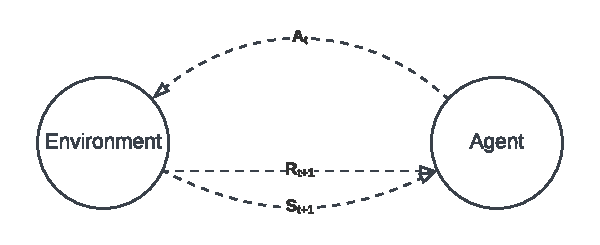
\includegraphics[width=0.6\textwidth]{papers/coordination2023/imgs/RL.pdf}
%     \caption{RL Framework}
%     \label{fig:rl}
%\end{figure}
In order for \ac{rl} to be effective, two conditions are fundamental: \emph(i) all is meant by \emph{goals/purposes/success} can be well thought of as the maximization of the expected 
    value of the cumulative sum of the reward (i.e., a scalar signal) -- called \emph{the reward hypothesis}; and \emph{(ii)} the environment state should summarize the past compactly, so that future states only depend on the current state (and not on past states) -- 
    \emph{the markov property}.

In literature, several algorithms can be used to solve \ac{rl} problems.
 In this work, we will focus on two of them: the \emph{Q-Learning}~\cite{Watkins1992} algorithm and 
 the \emph{Deep Q-Learning}~\cite{dqn} algorithm. 
The core part of both of these algorithms is the \emph{Q-function}, 
 which maps each state-action pair to a value that represents the expected future reward of taking that action in that state.
 Using a modified Bellman equation update, 
 the Q-function is iteratively updated based on the rewards received by the agent as it takes actions in the environment.
%
From the Q-function, 
 the agent can follow both an \emph{exploration} policy during the training phase and a \emph{behavioural} policy once the learning phase is complete. 
 The \emph{behavioural} policy is a greedy policy, 
 in which the agent chooses the action with the highest Q-value in a given state. 
 This policy ensures that the agent always chooses the best action to maximize its expected future reward. 
 On the other hand, during the exploration phase, 
 the agent uses an $\epsilon$-greedy policy, 
 where it chooses a random action with probability $\epsilon$
 and the best action (according to the Q-table) with probability 1-$\epsilon$. This allows the agent to explore the environment and learn from new experiences. 
 
 The main difference between the two algorithms is that in Q-Learning
  the Q-table is represented as a table, while in Deep Q-Learning it is approximated by a neural network.
 Therefore, the first approach works well for simple problems, 
  but it struggles to scale to complex problems due to the explosion of the state space; the second approach, on the other hand, addresses large-scaleness but requires much data to train the neural network.
 %To overcome this problem, the Deep Q-Learning~\cite{Mnih2015} was introduced, this algorithm 
 %uses a neural network to approximate the Q-table. The neural network takes 
 %as input the state and outputs the Q-values for each action.

 \begin{figure*}[t]
    \begin{subfigure}[b]{0.49\textwidth}
        \centering
        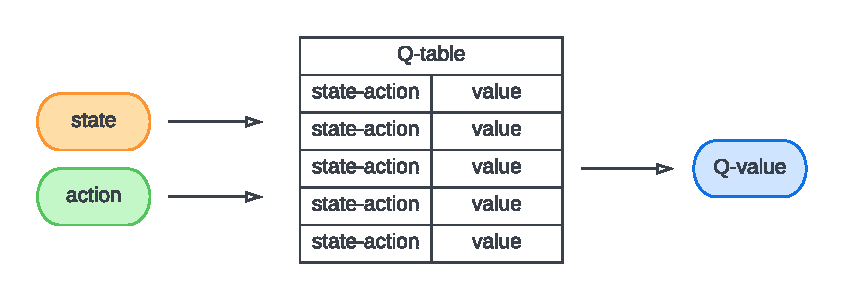
\includegraphics[width=\textwidth]{papers/coordination2023/imgs/q-learning.pdf}
        \caption{Q-Learning}
        \label{fig:ql}
    \end{subfigure}
    \begin{subfigure}[b]{0.49\textwidth}
        \centering
        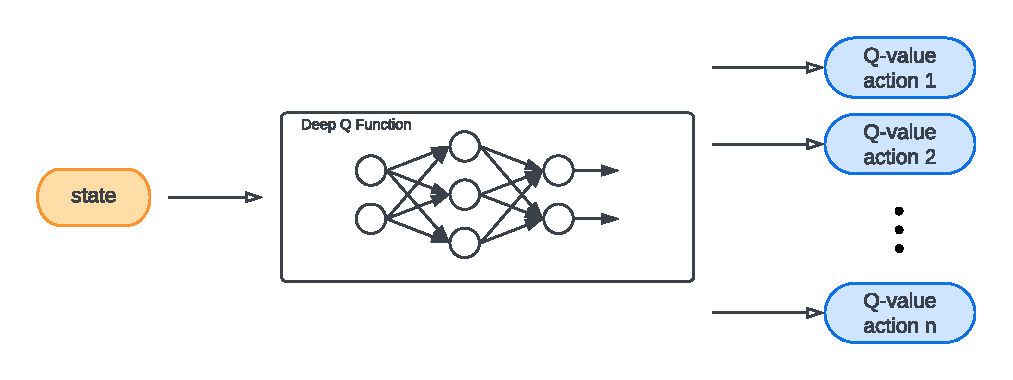
\includegraphics[width=\textwidth]{papers/coordination2023/imgs/deepQL.pdf}
        \caption{Deep Q-Learning}
        \label{fig:dqn}
    \end{subfigure}
\caption{Q-Learning and Deep Q-Learning visual comparison}\vspace{-10pt}
\end{figure*}


\subsection{Multi Agent Reinforcement Learning}
\ac{marl} is an extension of \ac{rl} where multiple agents 
 interact one another and with the environment. 
 Usually, \ac{marl} is modelled as a 
 \emph{Markov Game} (or Stochastic Game $\mathcal{S}$)~\cite{LITTMAN1994157} in which we have:
 \begin{itemize}
    \item A tuple $\mathcal{S} = <N, S, \{A^i\}, P, \{R^i\}>$ with $i \in 1 \dots N$
    \item The number of agents $N > 1$
    \item The action space of the i-th agent $A^i$. The global action space is defined as $\mathbb{A} = A^1 \times A^2 \times \dots \times A^N$
    \item A function describing the transition dynamics $P: S \times \mathbb{A} \rightarrow \mathcal{P}(S)$
    \item The reward function $R^i: S \times \mathbb{A} \times S \rightarrow \mathbb{R}$ for each agent $i$ 
 \end{itemize}

Based on the reward function used by the agents, MARL can be divided into two categories:
 i) \emph{cooperative}, where all the agents trying to maximize the same reward function (e.g., a group of robots trying to clean a room);
 ii) \emph{competitive}, where, potentially, each agent has its own reward function that is conflictual with the other (e.g., a rock-paper-scissor game).
 Cooperative MARL can be further divided into two additional categories (based on the policy),
 namely:
 i) \emph{homogeneous}, where all the agents have the same capabilities, i.e., they use the same policy
 ii) \emph{heterogeneous}, where each agent may have its own policy, in this case, each agent 
    tries to maximize the local policy following the global shared goal.   

In this work, we focus on a subset of MARL, namely: \emph{many-agent reinforcement learning}~\cite{yang2021many}. 
 The only difference between the two approaches is in the number of agents involved. Typically, in many-agent reinforcement learning the number of agents
 may range from a hundred to one or two thousands whereas, in Multi Agent Reinforcement Learning, there are only a few tens~\cite{smac,marl-curricula}.
 %(i.e., $N \gg 2$, typically less than one or two thousands ~\cite{smac,marl-curricula}).
 Moreover, we focus on cooperative homogeneous and heterogeneous learning.

\subsection{Alchemist}\label{alchemist}

Alchemist\footnote{\url{http://alchemistsimulator.github.io/}}~\cite{DBLP:journals/jos/PianiniMV13} is meta-simulator
 mainly designed for simulating complex distributed systems 
 in a rich variety of scenarios like swarm robotics~\cite{Casadei2021},
 large-scale sensor networks~\cite{Aguzzi_2022}, crowd simulation~\cite{Beal2015},
 path planning, and even morphogenesis of multi-cellular systems.

The simulator is \emph{meta} in nature, 
 as it is based on general abstractions 
 that can be mapped to specific use cases (i.e., \emph{incarnations}).
% 
Inspired by biochemistry, 
 the meta-model consists of a set of \emph{nodes} 
 that exist in an \emph{environment} and are linked together by \emph{relationship} rules. 
 Each node contains a sequence of \emph{molecules} and \emph{reactions}. 
%
 A \emph{molecule} represents a variable, 
 which acts as a container for data. 
 \emph{Reactions} instead are events that occur based 
 on a set of \emph{conditions}, 
 and are fired according to a time distribution, 
 producing an effect that is described as an action. 
This abstraction allows the simulator to be flexible 
 and adaptable to a variety of use cases and node numbers 
 (it could support thousands of nodes), 
 while maintaining a consistent underlying structure.

 The Alchemist simulator features four incarnations: 
  biochemistry, sapere, protelis, and \scafi{}, 
  each with a different way of modeling molecules and actions. 
The sapere incarnation uses a set of ground Linda-like tuples 
 to model concentration and has been used for crowd evacuation and resource discovery simulations. 
The protelis incarnation defines concentration as a Java Object and is commonly used in the literature for various simulations, 
 including crowd tracking and drone coordination. 
The \scafi{} incarnation supports the \scafi{} Scala DSL 
 and has been used in distributed peer-to-peer chats and situated problem-solving.

Alchemist offers an effortless method for loading simulations. 
 The process requires a YAML file that includes essential parameters, 
 such as the incarnation type, neighbour connection model, and node deployment. 
 In \Cref{fig:alchemist}, we have provided an example YAML file 
 that creates a simulation using the \scafi{} incarnation (first row). 
 It also defines the neighbourhood relationship based on fixed distances (0.5 in this case), 
 placing nodes in a fixed grid of size 10x10 starting at -(5,5) and ending at (5,5), 
 with a node-to-node distance of 0.25. 
 Finally, it loads the \scafi{} program called ``program'', 
 which is evaluated at each node with a frequency of 1. 
\begin{figure*}
\centering
\begin{subfigure}[b]{0.49\textwidth}
    \centering
    \begin{lstlisting}[language=yaml]
incarnation: scafi
network-model:
    type: ConnectWithinDistance
    parameters: [0.5]
deployments:
    type: Grid
    parameters: [-5,-5,5,5,0.25,0.25]
    /*dynamics of the simulation*/
    programs: 
        - program:
        - time-distribution: 1
            type: Event
            actions: 
            - type: RunScafiProgram
              parameters: [program]
        - program: send
\end{lstlisting}
\end{subfigure}
\hfill
\begin{subfigure}[b]{0.49\textwidth}
    \centering
    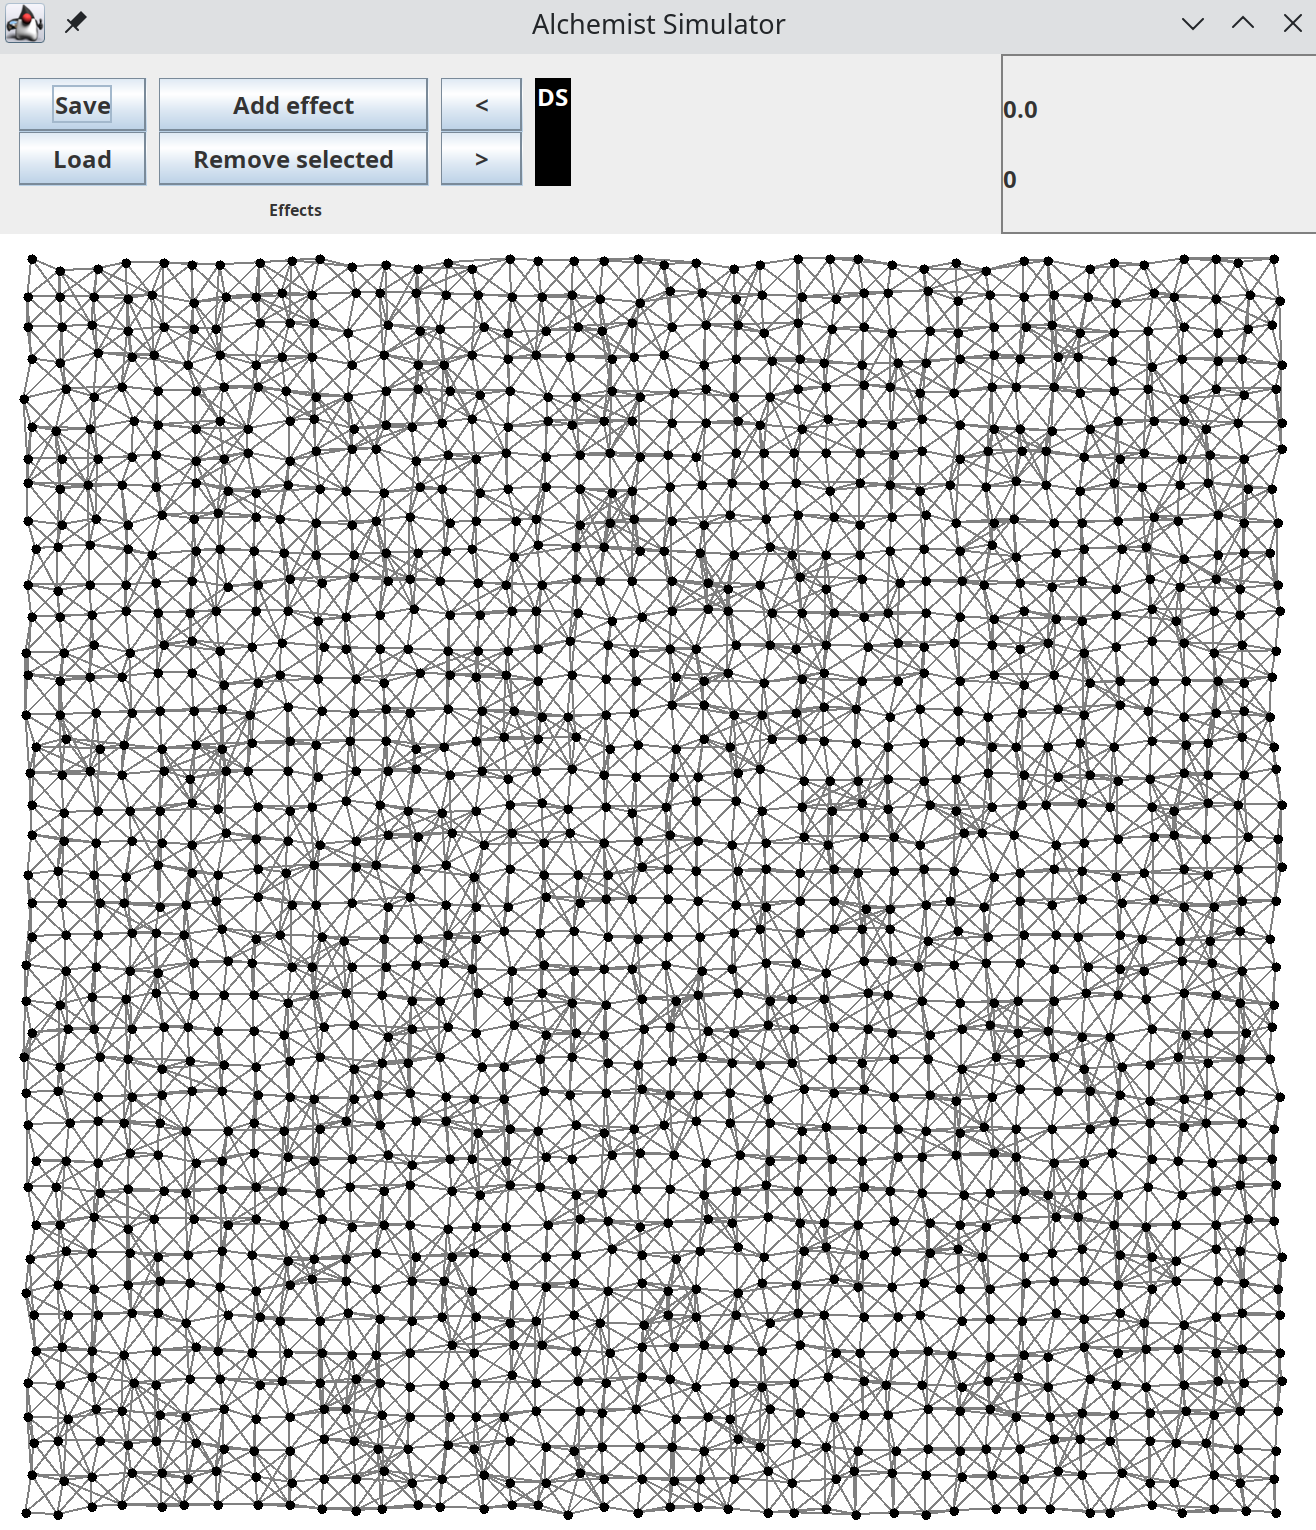
\includegraphics[width=\textwidth]{papers/coordination2023/imgs/alchemist.png}
\end{subfigure}
\caption[An Alchemist simulation example]{An Alchemist simulation example. 
    The simulation result on the right is obtained 
    by running the simulation described on the left.
    }
\label{fig:alchemist}
\end{figure*}

\subsection{ScaFi}\label{scafi}

\scafi{} (Scala Fields \footnote{\url{https://scafi.github.io/}})~\cite{Casadei2022} 
 is a Scala framework for developing large-scale 
 distributed applications and simulating systems of networked agents.
%
\scafi{} is designed for Aggregate Programming~\cite{Beal2015}, 
 which is a top-down global-to-local 
 macro-programming~\cite{Casadei2023} paradigm for distributed systems 
 where the focus is on the collective behaviour of the system 
 rather than on the individual agents that make up the system.
%
One of the unique features of aggregate computing 
 is its support for self-organizing systems -- that are systems 
 that can adapt to changes in the environment and 
 maintain their functionality without requiring centralized control.

In \scafi{}, agents are represented as nodes in a logical network, 
 and the interactions between agents are modelled 
 as the exchange of messages over edges in the graph.
%
\scafi{} provides a set of primitives for expressing distributed
algorithms, 
 which can all be interpreted as field-based coordination policies, namely, 
 distributed computations of maps from nodes to values (i.e. \emph{fields}).
 
  These primitives are designed to be composable and reusable, 
 allowing programmers to build complex distributed algorithms from simple building blocks.
%
%ScaFi includes a simulator for testing and evaluating the behavior of
%distributed algorithms under different conditions. The simulator allows
%programmers to simulate large-scale distributed systems and to observe
%how the system behaves under different scenarios. The simulator also
%provides tools for visualizing the behavior of the system and for
%analyzing the performance of the algorithms. 
%This is achieved through the use of distributed
%algorithms that enable agents to communicate and coordinate with each
%other in a decentralized manner.

%ScaFi has been used in various domains, including sensor networks,
%social networks, and robotics, among others. It is an open-source
%project and is actively maintained by researchers from various
%universities and research institutions.

\section{\scarlib{}}\label{contribution}
%\meta{This section should provide a description of the framework, including the main features and the architecture.}
%\newline
%\begin{itemize}
%    \item Main features
%    \item Library Modules schema and discussion
%    \item Core module architecture
%    \item Alchemist-Scafi module architecture
%    \item CTDE and DTDE schema
%\end{itemize}

\scarlib{} \footnote{Tool available on GitHub at \url{https://github.com/ScaRLib-group/ScaRLib}}~\footnote{demo video at: \url{https://github.com/ScaRLib-group/ScaRLib-demo-video}} is a research Scala framework designed to support
the development of \ac{cmarl} systems by JVM-based high-level specification, and with learning performed under the hood by PyTorch\footnote{\url{https://pytorch.org/}}.
%
This project aims to provide a tool that allows easy and powerful system specification.
%
To meet this purpose we have designed many abstractions, that model high-level aspects of the MARL domain, 
 without caring about low-level implementation details.
Basically, \scarlib{} is composed of three main modules (\Cref{fig:modules}), namely: 
    i) \texttt{scarlib-core} that implements the main abstractions over the CMARL domain,
    ii) \texttt{dsl-core} that provides a high-level language to specify the system, and
    iii) \texttt{alchemist-scafi} that provides bindings between \scarlib{} and the two tools Alchemist and \scafi{}.
    It is important to note that \scarlib{} is not limited to the Alchemist-\scafi{} combination, that module is 
    already implemented due to the actual need, however, it is possible to implement other bindings to other tools
    (e.g., by replacing Alchemist with some other simulator, for example, FLAME GPU~\cite{flame}).
\begin{figure}[t]
    \centering
    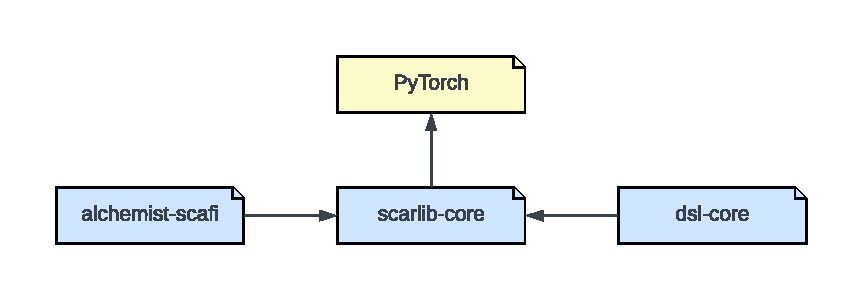
\includegraphics[width=0.7\textwidth]{papers/coordination2023/imgs/scarlib-modules.pdf}
    \caption{\scarlib{} main modules}
    \label{fig:modules}
\end{figure}

\paragraph{Core abstraction:} the module \texttt{scarlib-core} implements the core functionalities and abstractions of the framework, such as the definition of the main data structures and the implementation of the main algorithms. 
%
All the abstractions (\Cref{fig:arc}) are built around a bunch of concepts. The key element is the \texttt{System}, which is a collection of agents that interact within a shared environment and that are trained to optimize a global or local reward signal
expressed by a reward function. 
%
The tool comes with two types of systems already implemented that are very common in literature~\cite{Du2020},
i.e., centralized training and decentralized execution (\texttt{CTDESystem}) and decentralized training and execution (\texttt{DTDESystem}).
Furthermore, an implementation of the DQN algorithm \cite{Mnih2015} is provided and used to train agents. 
The end-user who wants to run a learning process only has to implement four elements
in order to define his own system with the desired collective goal, which are: 
 i) the environment, 
 ii) the agent state space, 
 iii) the action space and,
 iv) the reward function.
Only by using this module, 
 it is possible to run a simple learning process in a simulated environment based on our platform.

\begin{figure}[t]
    \centering
    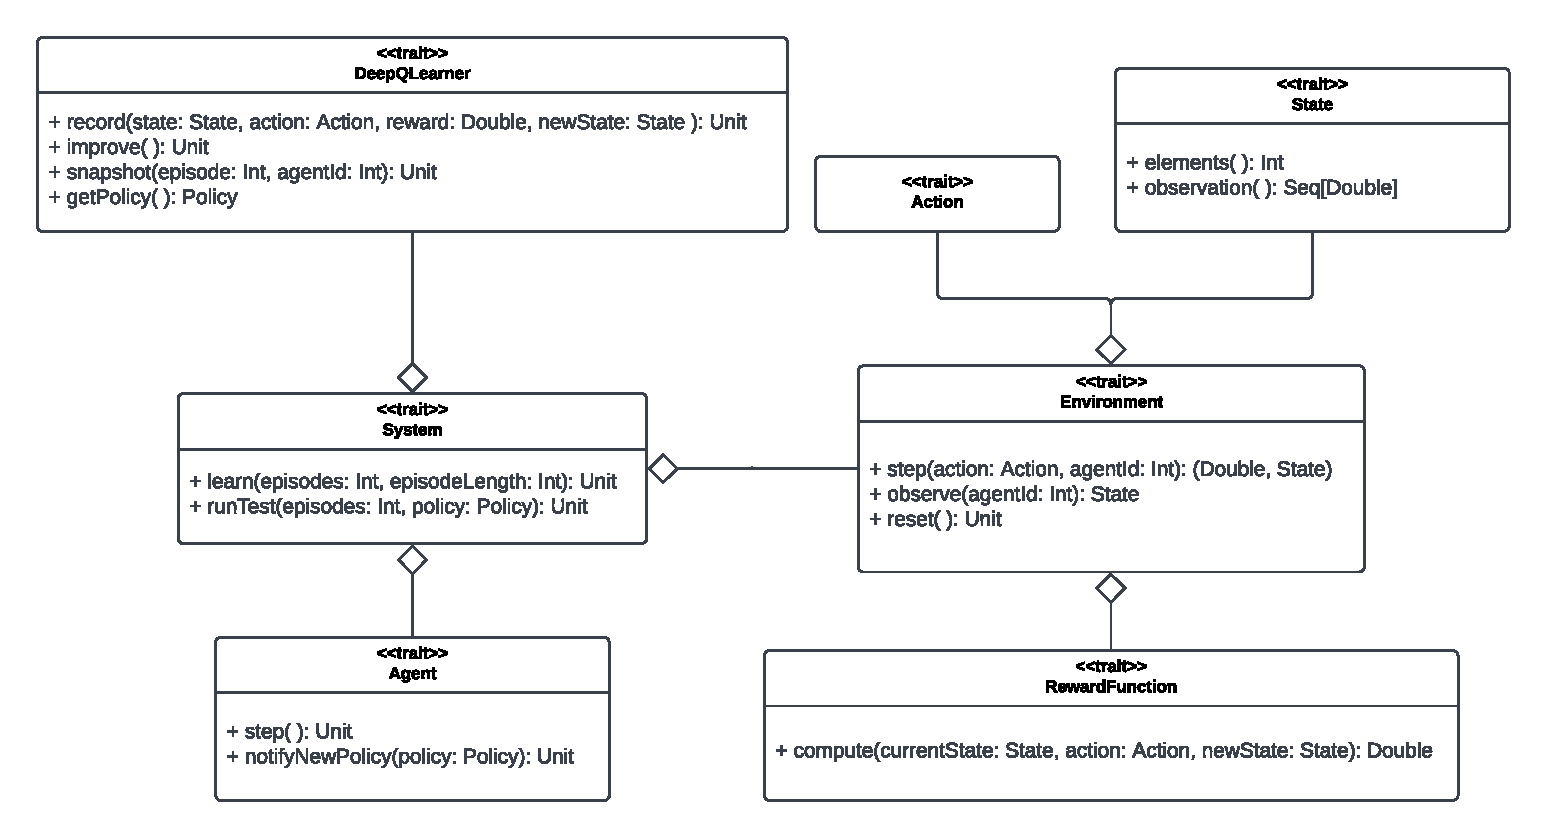
\includegraphics[width=\textwidth]{papers/coordination2023/imgs/core-architecture.pdf}
    \caption{\scarlib{} core architecture}
    \label{fig:arc}
\end{figure} %% TODO increase the font in this figure

To better understand the dynamics of the system it is useful to explain some internals.
%
Both systems utilize a training process that consists of multiple \emph{epochs}, 
 with each epoch comprising a set of \emph{episodes}. 
 During each episode, 
 the agents receive the current state as input and 
 execute an action based on that state. 
This collective action causes 
 the environment to move to the next state, 
 advancing the simulation to the next episode.
At the end of an epoch, 
 the environment is reset, and the agents are trained using the collected experience.

Most specifically,
 if the chosen system is a \texttt{CTDESystem} (\Cref{fig:ctde}) the agents are trained in a centralized way, 
 for that reason, there is  a single central dataset, 
 where the global experience of all the agents is stored, 
 and a single central learner that is responsible for the training process 
 and for the improvement of the policy neural network.
% 
The system is also responsible 
 for the execution of all the agents and the notification of the updated policy. 
 In this way, it is possible to easily extend the system in order to modify the execution flow, e.g., if a concurrent and distributed execution is needed. 
%
The \texttt{DTDESystem} (\Cref{fig:dtde}) works similarly, 
 the only difference is that every agent has its own dataset and learner.

%In order to provide an efficient learning process we have bindings with a state-of-the-art 
% deep learning library, namely: PyTorch \footnote{\url{https://pytorch.org/}}.
% Those bindings are provided by another library called ScalaPy \footnote{\url{https://scalapy.dev/}} 
% and allows the end-user to train the models both on CPUs and GPUs.

Regarding the training process,
 since the tool aims to support neural-network-based RL algorithms (like DQN),
 we chose to use the current de facto standard framework 
 for building neural networks, which is PyTorch---alternatives include DL4J~\footnote{\url{https://deeplearning4j.konduit.ai/}}, which could be subject of future investigation.
 
%
One way to integrate this library into a JVM environment could be 
 to rely on its native core (LibTorch) using JNI -- 
 as was done in \texttt{scala\_torch}~\footnote{\url{https://github.com/microsoft/scala_torch}} project. 
 In \scarlib{}, we chose a convenient approach 
 that allowed us not only to access PyTorch 
 but also all the libraries connected to it 
 (e.g., torch geometric, etc.), 
 which is to use ScalaPy~\cite{Laddad2020}  to interact directly with the Python API 
 of these libraries.
%
This integration generally involves:
i) setting up a Python environment in which the libraries of interest are instantiated, and
ii) creating a Scala API that isolates what is necessary to access the Python ecosystem.
In this case, we have isolated everything in DQN, which is therefore the entry point for accessing Torch.
\begin{figure*}[t]
    \centering
    \begin{subfigure}[b]{0.49\textwidth}
        \centering
        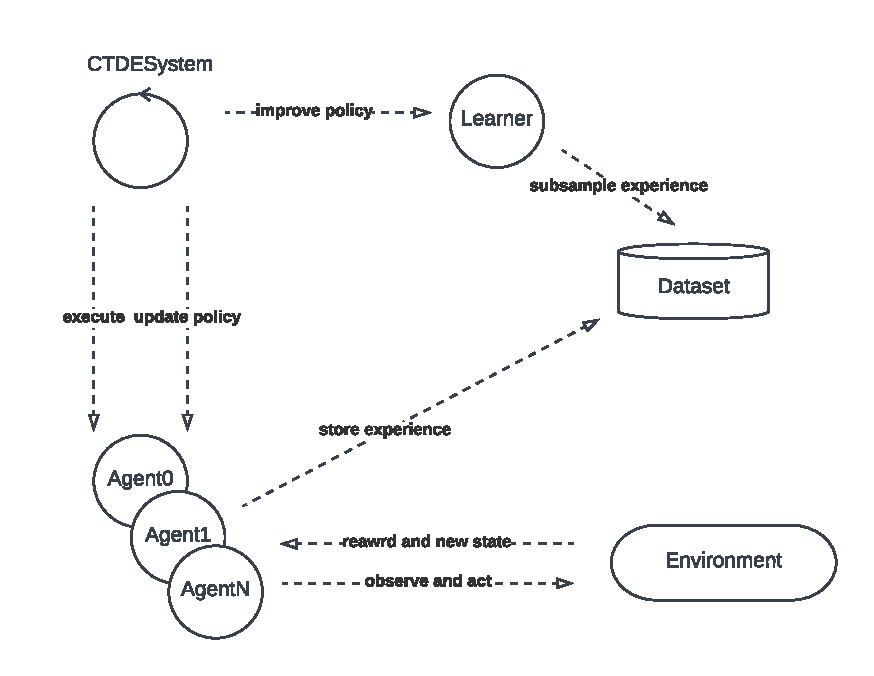
\includegraphics[width=\textwidth]{papers/coordination2023/imgs/ctdesystem.pdf}
        \caption{CTDE System}
        \label{fig:ctde}
    \end{subfigure}
    \begin{subfigure}[b]{0.49\textwidth}
        \centering
        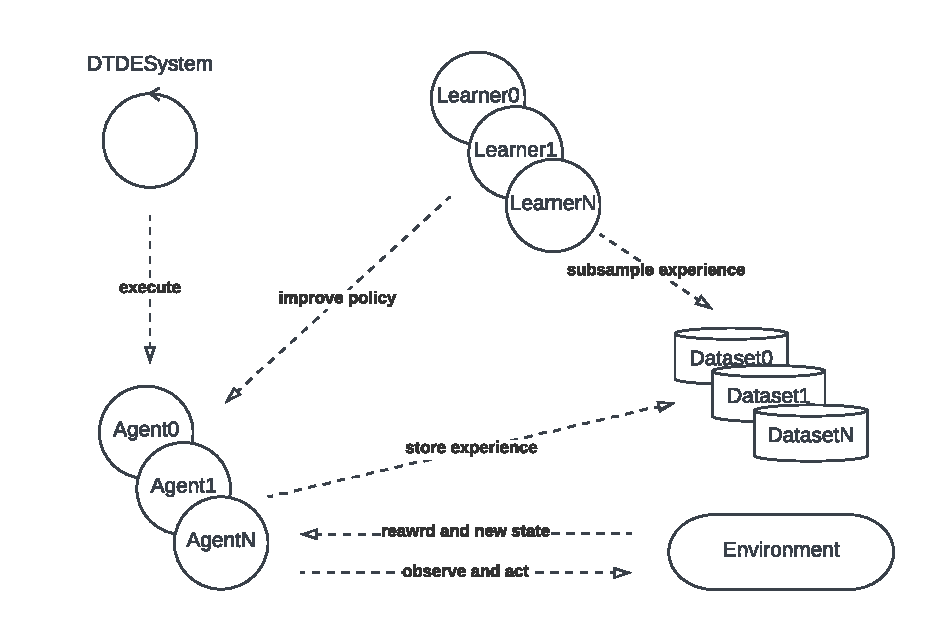
\includegraphics[width=\textwidth]{papers/coordination2023/imgs/DTDE.pdf}
        \caption{DTDE System}
        \label{fig:dtde}
    \end{subfigure}
\caption[Examples of developed System dynamics in \scarlib{}]{Examples of developed System dynamics. 
On the left, there is the centralized system, 
where a learner with a global view of the system 
updates the policy shared with all agents. 
%
On the right, there is a decentralized system, 
where each agent has a local policy and a local policy.}
\end{figure*}

\paragraph{\scafi{}-Alchemist integration:} in addition to the core, we have implemented another module called \texttt{alchemist-scafi} (\Cref{fig:alchemist-arc}) 
 in which there is the integration with the two tools: 
 Alchemist \cite{DBLP:journals/jos/PianiniMV13} and \scafi{} \cite{Casadei2022}.
%
Such integration enables the possibility to run the learning process 
 in an aggregate computing context.
This is a key part of this contribution. 
 In fact, although Alchemist has been used for \ac{cmarl} with \scafi{} in the past~\cite{Aguzzi2022,DBLP:conf/acsos/AguzziCV22}, 
 ad-hoc solutions were always created that were difficult to \emph{reuse}, 
 \emph{rigid}, \emph{untested}, and had \emph{interoperability issues} between Alchemist 
 and the chosen native libraries.
With this integration, 
 we want to provide a usable system once and for all, 
 to bring the Many-agent RL community closer 
 to the use of this simulator and this paradigm, 
 which has proven flexible in describing the most diverse environments -- 
 from robotic swarms~\cite{Casadei2021} to data centres.

The specification of a learning system does not change, only two new elements are added: 
 the specification of the Alchemist simulation and the implementation of the \scafi{}-based logic.
%
In particular, 
 the Alchemist simulation will be defined as shown in \Cref{fig:alchemist}, 
 by passing a \scafi{} class as a program, which contains aggregate programming code. 
 In order to advance the training process, 
 a molecule with the current action to be taken (a subtype of \texttt{Action} class) 
 will be present in the \scafi{} program. 
 This will be injected by a learner that contains the \ac{rl} policy.
 Moreover, the aggregate program will evaluate 
 the environment state (which must be a subtype of \texttt{State})
 using \texttt{computeState} 
 and insert it into the \texttt{state} molecule, that will be 
 used by the learner to update the policy.
\begin{figure}[t]
    \centering
    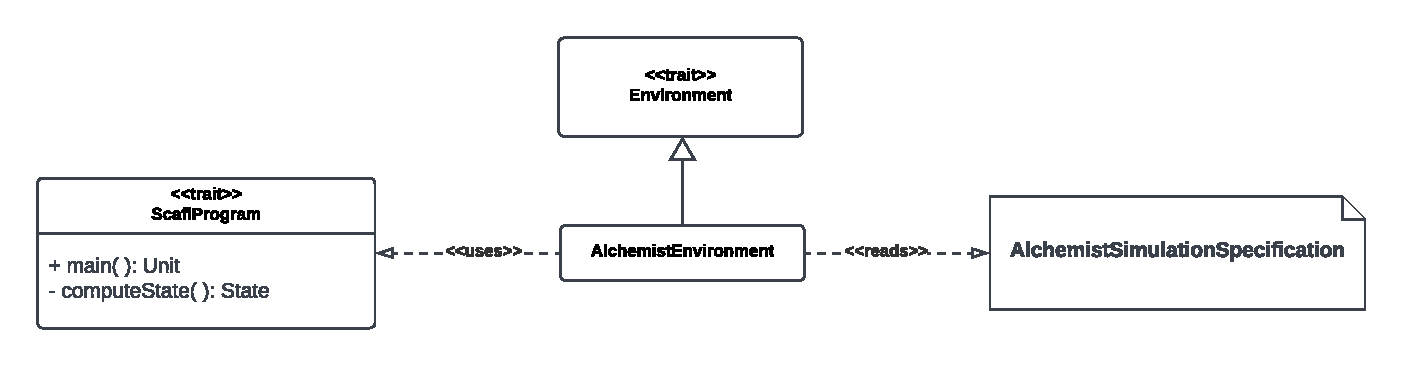
\includegraphics[width=\textwidth]{papers/coordination2023/imgs/alchemist-scafi-arc.pdf}
    \caption[\scarlib{} \texttt{alchemist-scafi} architecture]{\scarlib{} \texttt{alchemist-scafi} architecture. 
    A \texttt{ScafiProgram} should be passed to the \texttt{AlchemistEnvironment}
    in order to start the learning process. 
    }
    \label{fig:alchemist-arc}
\end{figure}

\paragraph{DSL for learning configurations:} 
the latest module developed
 is an internal DSL that allows for agile 
 and flexible creation of \ac{cmarl} training systems. 
 We made this choice to bridge the gap between the \ac{marl} system designer's 
 idea and the actual training system. 
 Additionally, by using a system like Scala, 
 creating a typed \ac{dsl} allows for capturing errors during compilation, 
 rather than waiting for the actual system runs 
 to intercept simple configuration errors.

The exposed \ac{dsl} is a simple facade 
 to the abstractions shown in the \texttt{scarlib-core} module. 
Therefore, if a developer wants to start their simulation 
 (let's say in Alchemist), 
 they must first define a reward function that indicates 
 how good the current state of a certain agent 
 is compared to the current environmental condition.
\begin{lstlisting}
class MyRewardFunction extends CollectiveRewardFunction:
    override def computeReward(state: State, action: Action, nextState: State): Double = ...
\end{lstlisting}
Consequently, they must decide which actions are supported 
 by the agents living in the chosen system. 
%
Since we are talking about \ac{cmarl} systems, 
 we suppose that each agent has the same action space. 
 Thus, it is possible to define a set of actions as a product type:
\begin{lstlisting}
sealed trait MyAction extends Action
object MyAction:
    case object A extends MyAction
    case object B extends MyAction
    case object C extends MyAction
    def all: Seq[MyAction] = Seq(A, B, C)
\end{lstlisting}
Final refinements required include: 
i) choosing the class of the Alchemist environment to instantiate, 
ii) defining the number of agents living in the chosen environment, and 
iii) defining the size of the buffer in which the memory will be stored,
expressed as follows:
\begin{lstlisting}
val system = learningSystem {
    rewardFunction { new MyRewardFunction() }
    actions { MyAction.all}
    dataset { ReplayBuffer[State, Action](10000) }
    agents { 50 } // select the number of agent
    environment {
        // select a specific environment
        "it.unibo.scarlib.experiments.myEnvironment"
    }
}
\end{lstlisting}
%The last module: \texttt{dsl-core}, provides a handy way for defining the learning system. 
%Basically, it is composed of six composable elements, an example is provided in \ref{lst:sysdef}.

%begin{lstlisting}[caption={CTDE system definition} ,label={lst:sysdef},language=scala]
%val system = learningSystem {
%    rewardFunction { new CohesionRewardFunction() }
%    actions { CohesionActions.toSeq() }
%    dataset { ReplayBuffer[State, Action](10000) }
%    agents { 50 }
%    environment {
%        "it.unibo.scarlib.experiments.CohesionEnvironment"
%    }
%}
%\end{lstlisting}
\paragraph{Tool usage:}

the tool is published on Maven Central 
 and it is possible to include it in your project, 
 for example, through a build system. 
 In the case of Gradle, for instance, 
 you will need to add the following instructions:
\begin{lstlisting}
implementation("io.github.davidedomini:scarlib-core:1.5.0")
implementation("io.github.davidedomini:dsl-core:1.5.0")
\end{lstlisting}
%
At this point, it will be possible to create 
 your own training system as shown in the DSL section. 
 To start the training, you will then need to write:
\begin{lstlisting}
learningSystem.train(episodes = 1000, episodeLength = 100)
\end{lstlisting}
%
Of course, 
 the system can also be used to verify a certain 
 policy that has been learned during a training process. 
% 
To do this, first, 
 you will need to load the neural network extracted during training:
\begin{lstlisting}
val network = PolicyNN(path, inputSize = ..., hiddenSize = ...)
\end{lstlisting}
Then you can execute the test in the following way:
\begin{lstlisting}
system.runTest(episodeLength = 100, network)
\end{lstlisting}
For further details on how to specify simulations and environments, 
 please refer to the repository README, 
 the presentation video and 
 the developed simulation (following section).
\section{Experiments}\label{experiments}
% \meta{This section should provide a description of the experiments, including the results and the discussion.}
% \meta{For each experiment, we can have the following structure:
% \paragraph{Description}
% Here you should describe the experiment, including the environment, the agents, the algorithm, etc.
% \paragraph{Results}
% Here you should show the result of the experiment, including the plots and the discussion.
% }

%\subsection*{Cohesion and Collision}
\paragraph{Description}
%This environment consists of a group of agents (in our experiment fifty) that interact in a 2D world 
% to learn how to stay close with each other without colliding. 
%Each agent has a fixed neighborhood (the three closest, that is an hyper-parameter) 
% and can perform eight actions, namely: north, south, east, 
% west, north-east, north-west, south-east and south-west. 
% The state of each agent consist of the relative distance to the neighborhood 
%  and of his own position.
%The reward function (\Cref{fig:cc-rf}) is parametrized by a target distance $d$, in the graph the target
% distance is represented by the red vertical line.
% The portion of the graph to the right of the red line represents the influence of the cohesion term:
% the more the agents are far from each other, the more the reward linearly decrease.
% Instead, the portion of the graph to the left of the red line represents the influence of the 
% collision term: if the agents are too close to each other, the reward function 
% has an exponential decreasing trend. 
To test ScarLib's functionality, 
 we develop an experiment~\footnote{repository available at \url{https://github.com/ScaRLib-group/ScaRLib-flock-demo}}
 involving a relatively large number of agents 
 and non-trivial coordination tasks. 
% 
We aim to create a flock of drones 
 that moves to avoid collisions with each others, by learning a policy by which each 
 agents decide how to move based on neighbours relative position.
% 
This is a well-known problem, and various models and algorithms exist which we draw upon \cite{DBLP:conf/siggraph/Reynolds87,inverserl}. %% todo add citations
% and learning processes exist. % I'd try not to say this... or just discuss it in related works
%
In this case, %%
 we assumed that agents position themselves in an unlimited 2D environment 
 with a fixed neighbourhood (the closest five, in our experiments, though this is a simulation parameter)
 and have the ability to perform movement steps in the 8 directions of a square grid (horizontally, vertically, or diagonally).
%
The environment state, as perceived by the single agent, is the relative distance to the closest neighbours.
%
Particularly, it was expressed through \scafi{} as:
\begin{lstlisting}
val state = foldhoodPlus(Seq.empty)(_ ++ _)(Set(nbrVector))
\end{lstlisting}
where \texttt{nbrVector} is the vector representing the relative position of the neighbour.
\lstinline|foldhoodPlus| is a \scafi{} function that allows to fold over the neighbourhood 
 and \lstinline|++| is the concatenation operator for sequences.

The crucial point for this task is
 the definition of the reward function. 
 In this simulation, we based it on \emph{collision} and \emph{cohesion} factors. 
%
We aim to learn a policy by which agents, initially spread in a very sparse way in the environment, move toward each other until reaching approximate $\delta$  distance without colliding, ultimately forming one or many close groups.
%
%Most specifically, the action taken by an agent is expressed as a movement towards the (closest) neighbour with maximum distance: what we want to learn is the distance to be travelled.

The collision factor comes into play when the distance is less than $\delta$, 
 and exponentially weighs the distance $d$ relative to its closest neighbour:
\begin{equation}
    \label{eq:collision-factor}
    \begin{split}
        \text{collision} = \begin{cases}
            0 & \text{if } d > \delta \\
            \exp\left(-\frac{d}{\delta}\right) & \text{otherwise}
        \end{cases}
    \end{split}
\end{equation}
In this way, when the negative factor is taken into account: 
 the system will tend to move nodes away from each other.

However, if only this factor were used, 
 the system would be disorganized. 
 This is where the cohesion factor comes in. 
 Given the neighbour with the maximum distance $D$, 
 it linearly adjusts the distance relative to the node being evaluated by function:
\begin{equation}
    \text{cohesion} = \begin{cases}
        0 & \text{if } d < \delta \\
        -(D - \delta) & \text{otherwise}
    \end{cases}
\end{equation}
%
The overall reward function is defined as the sum of these two factors ($cohesion + collision$)
 as shown in \Cref{fig:cc-rf}.
 \begin{figure}[t]
    \centering
    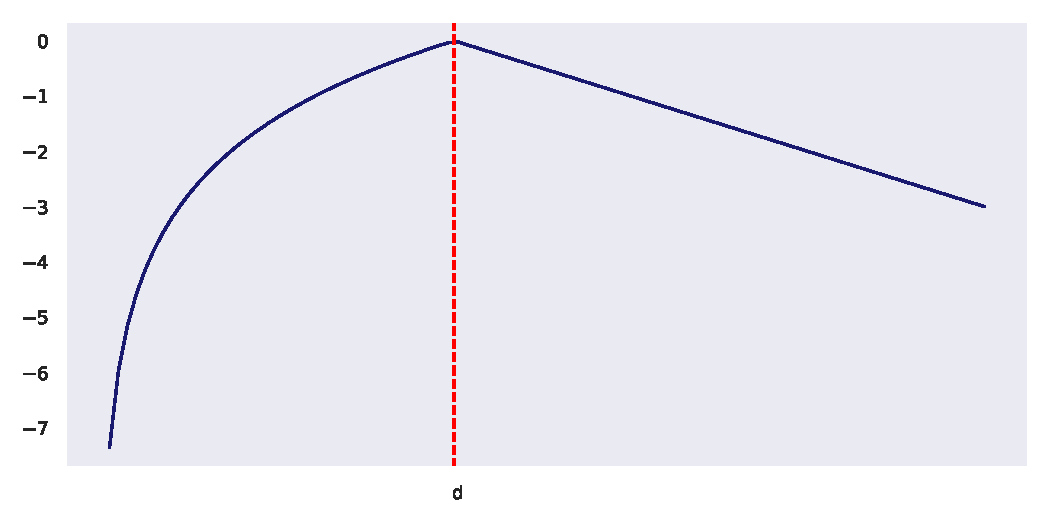
\includegraphics[width=0.6\textwidth]{papers/coordination2023/imgs/ccreward.pdf}
    \caption[cohesion collision reward function]{Cohesion-Collision reward function: the red vertical line represents the target distance $d$.
        The portion of the graph to the right of the red line represents the influence of the cohesion term,
        while the left one represents the influence of the collision term.
    }
    \label{fig:cc-rf}
\end{figure}


\paragraph{Results}
%\Cref{fig:cc-results} shows the results of the two experiments, the first one ran with 25 agents (purple lines)
%    and the second one with 50 agents (cyan lines) using a hundred and fifty episodes each of two hundred steps.
% The first graph (\Cref{fig:loss-cc}) shows a comparison of the loss functions,
%  while the second one of the reward functions. 
%  In both learning processes, 
%  when the loss function increases, 
%  the reward function decreases, 
%  which is to be expected as they are inversely proportional. Additionally, both cases exhibit similar 
%  inflexion points despite differences in the agents used, and convergence is achieved in both cases after around 
%  75 episodes.
%  The results are consistent with the predictions and the outcome 
%  does not vary significantly with a different number of agents.
To verify the functionality of the described simulation, 
 we divided the evaluation into two parts. 
%
In the first part, 
 we trained the system for a total of 1000 epochs, 
 each consisting of 100 episodes (or steps). 
%
For each epoch,
 we randomly place 50 agents in a grid large 50x50 meters.
 We set the target distance $\delta$ at 2 meters.

Given the flexibility of \scarlib{}, 
 we tested the training with both CDTE and DTDE processes 
 to ensure that the system could produce policies 
 capable of solving the described task in both cases. 
% 
With the homogeneous policies found (i.e., the one extracted from the CTDE process), 
 we verified that the system's behaviour 
 was consistent with what was learned by varying the initial seed 
 in 16 simulations
%
With the CDTE policy, 
 since we considered the system homogeneous, 
 we also verified the behaviour as the number of nodes varied,
 expecting similar performance as the nodes increased.

The graphs shown in \Cref{fig:cc-results} 
 demonstrate the multi-objective nature of the problem. 
In fact, cohesion and collision are two contrasting signals, 
 and the system had to find a balance between these two values. 
 The graphs show that DQN can generally optimize one signal at a time, 
 with cohesion tending towards zero and collision increasing. 
% 
Nonetheless, after 500 epochs in CTDE simulation,  
 we see that the system had already found a balance between these two factors.
%
In the case of DTDE learning, 
 we observe that convergence is achieved in fewer steps (\~ 50). 
 This is because there is a greater number of policies and 
 therefore greater overall complexity compared to a single homogeneous policy.

During the testing phase 
 (\Cref{fig:simulation-snapshots} shows a series of snapshots of the learned policy), 
 we observed that the system is capable of maintaining a distance of approximately $\delta$, 
 both in the CDTE and DTDE cases. 
 Most specifically, 
 we note that the homogeneous policy is generally 
 a winning choice for homogeneous \ac{cmarl} tasks. 
%
Increasing the number of agents (from 50 to 200), 
 we can observe that collective performances are similar to those with few agents (\Cref{fig:test}).
\begin{figure*}[t]
    \centering
    \begin{subfigure}[b]{0.32\textwidth}
        \centering
        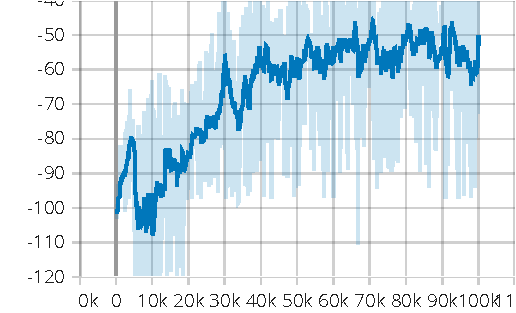
\includegraphics[width=\textwidth]{papers/coordination2023/imgs/reward-ctde.pdf}
        %\caption{Total average reward}
        %\label{fig:reward-cc}
    \end{subfigure}
    \hfill
    \begin{subfigure}[b]{0.32\textwidth}
        \centering
        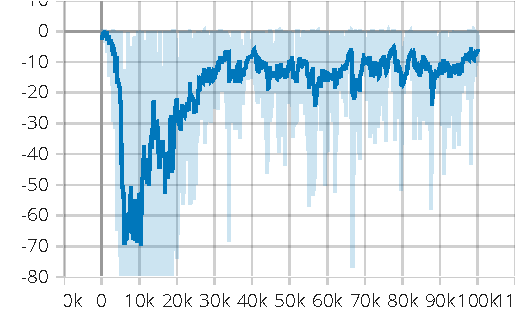
\includegraphics[width=\textwidth]{papers/coordination2023/imgs/collision-ctde.pdf}
        %\caption{Average collision factor}
        %\label{fig:collision-cc}
    \end{subfigure}
    \hfill
    \begin{subfigure}[b]{0.32\textwidth}
        \centering
        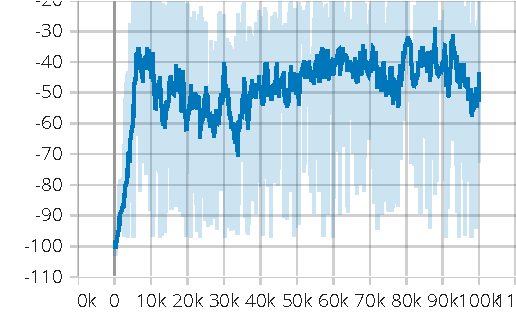
\includegraphics[width=\textwidth]{papers/coordination2023/imgs/cohesion-ctde.pdf}
        %\caption{Average cohesion factor}
        %\label{fig:cohesion-cc}
    \end{subfigure}
    \par\bigskip
    \begin{subfigure}[b]{0.32\textwidth}
        \centering
        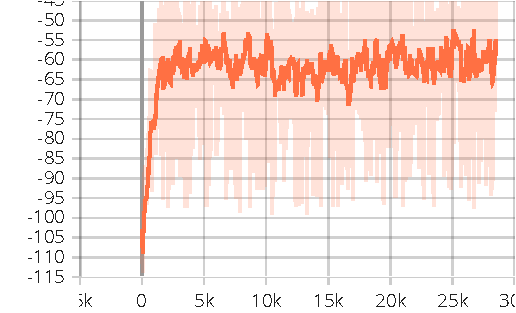
\includegraphics[width=\textwidth]{papers/coordination2023/imgs/reward-dtde.pdf}
        \caption{Total average reward}
        \label{fig:reward-dcc}
    \end{subfigure}
    \hfill
    \begin{subfigure}[b]{0.32\textwidth}
        \centering
        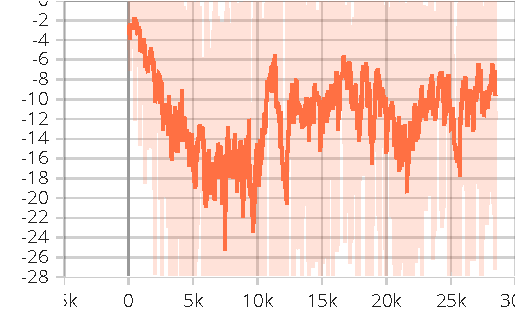
\includegraphics[width=\textwidth]{papers/coordination2023/imgs/collision-dtde.pdf}
        \caption{Average collision factor}
        \label{fig:collision-dcc}
    \end{subfigure}
    \hfill
    \begin{subfigure}[b]{0.32\textwidth}
        \centering
        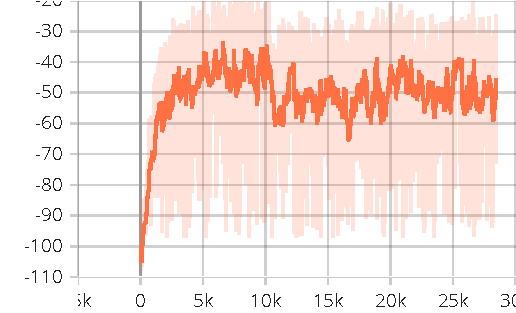
\includegraphics[width=\textwidth]{papers/coordination2023/imgs/cohesion-dtde.pdf}
        \caption{Average cohesion factor}
        \label{fig:cohesion-dcc}
    \end{subfigure}
\caption[Cohesion and collision experiment results]{Cohesion and collision experiment results. The y-axis represents the reward value.
The x-axis represents the total number of episodes.
The first three graphs show the results of the CDTE learning process, while the last three show the results of the DTDE learning process.}
\label{fig:cc-results}
\end{figure*}

\begin{figure*}[t]
    \centering
    \begin{subfigure}[b]{0.25\textwidth}
        \centering
        \fbox{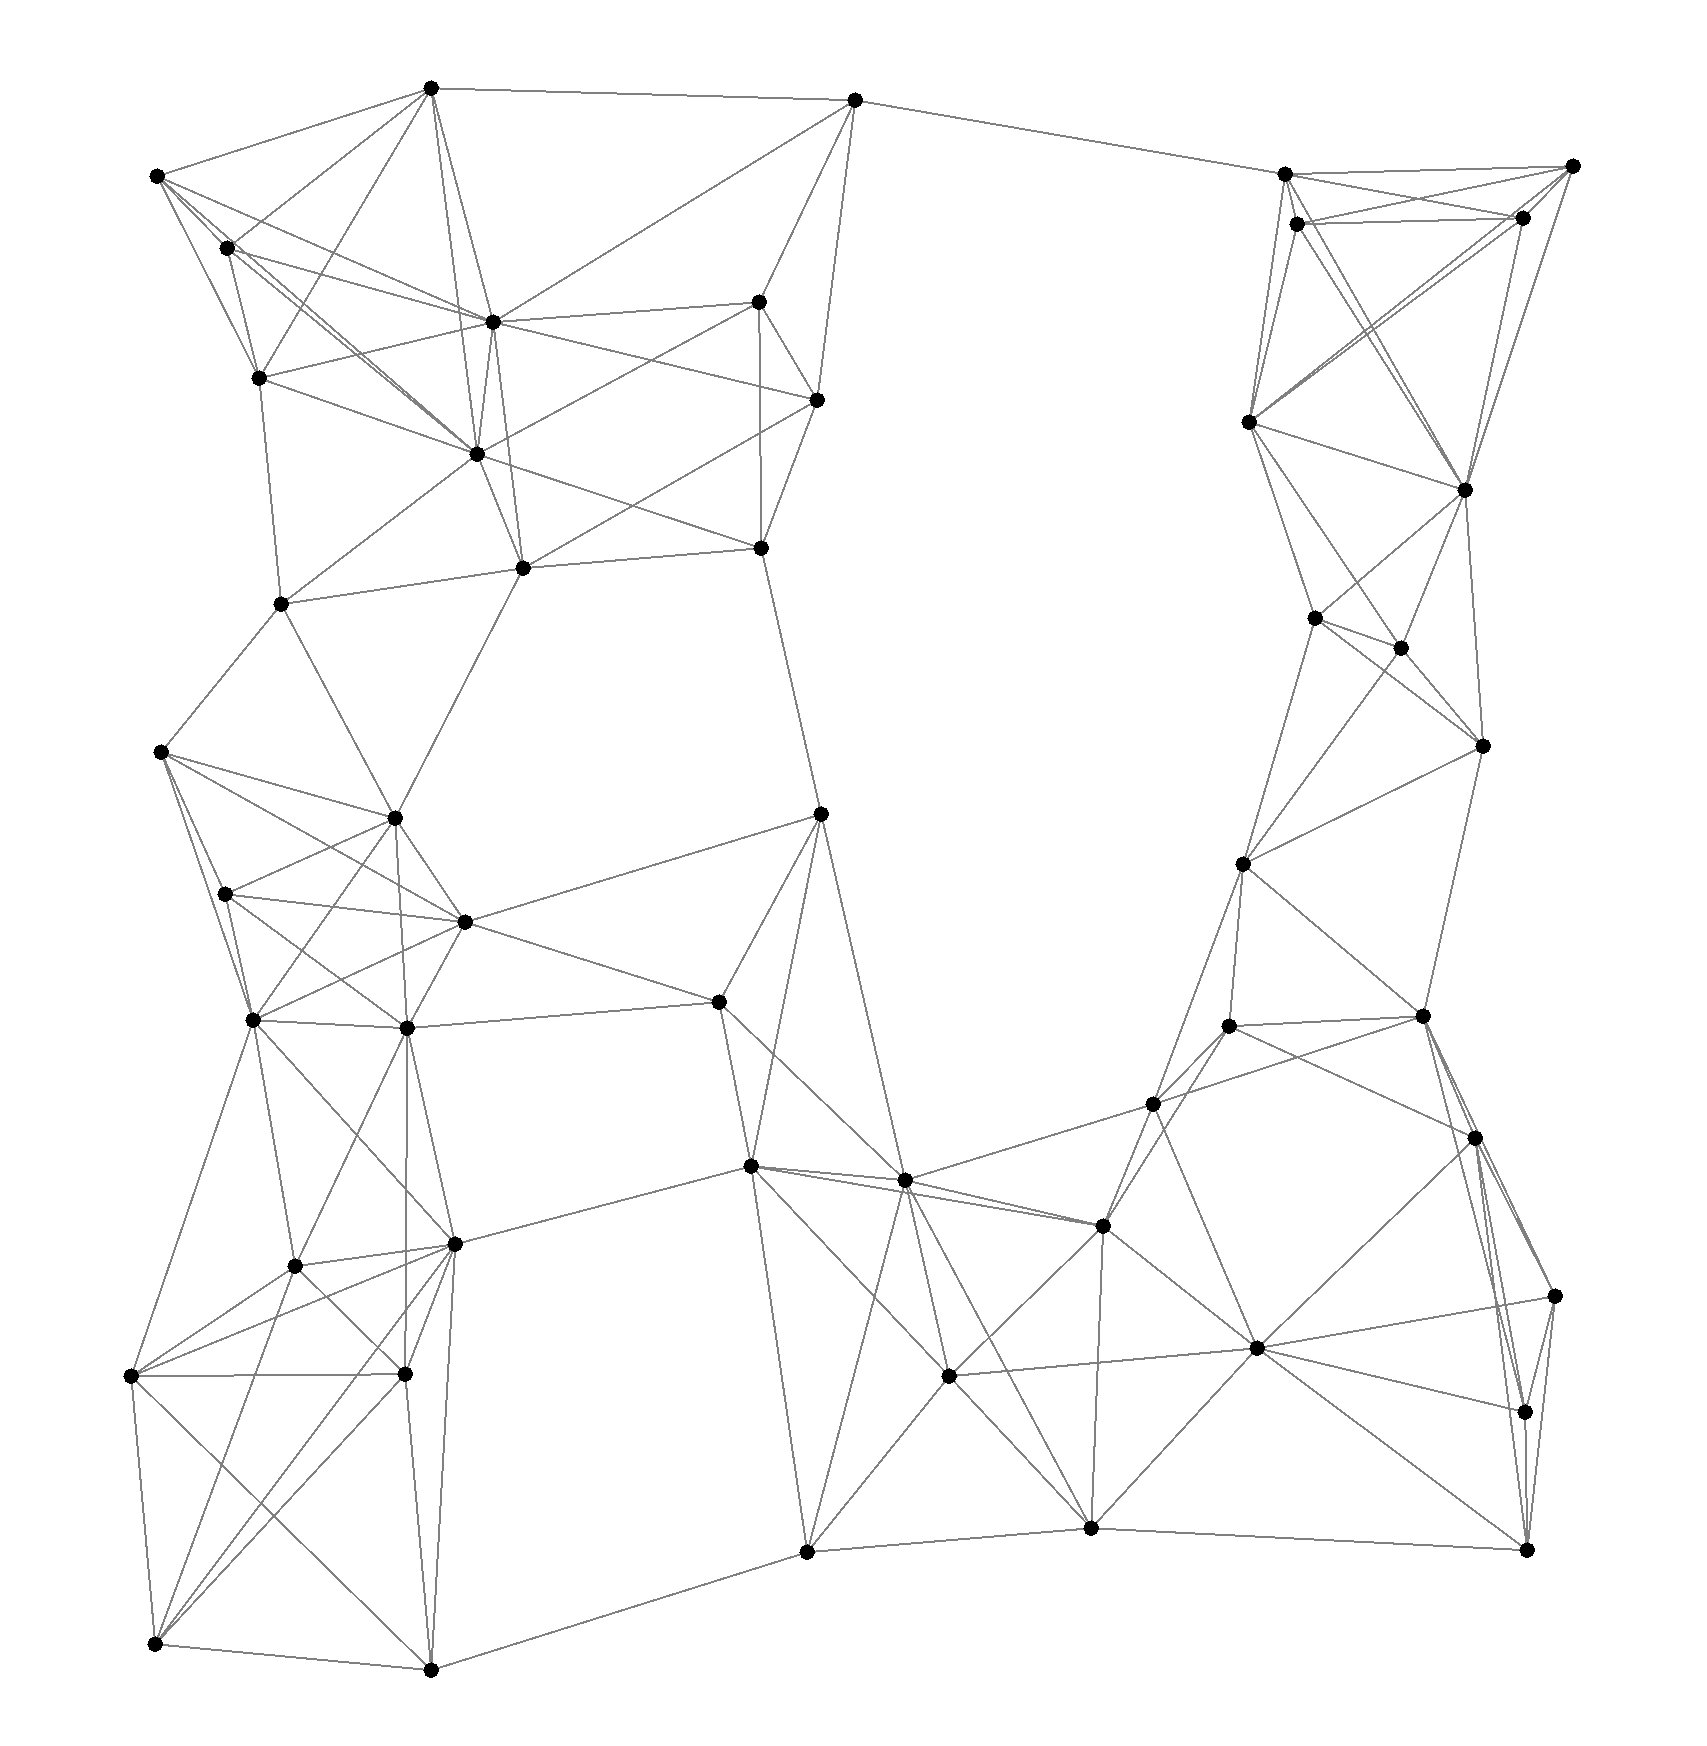
\includegraphics[width=\textwidth]{papers/coordination2023/imgs/1.png}}
        \caption{}
    \end{subfigure}
    \hfill
    \begin{subfigure}[b]{0.25\textwidth}
        \centering
        \fbox{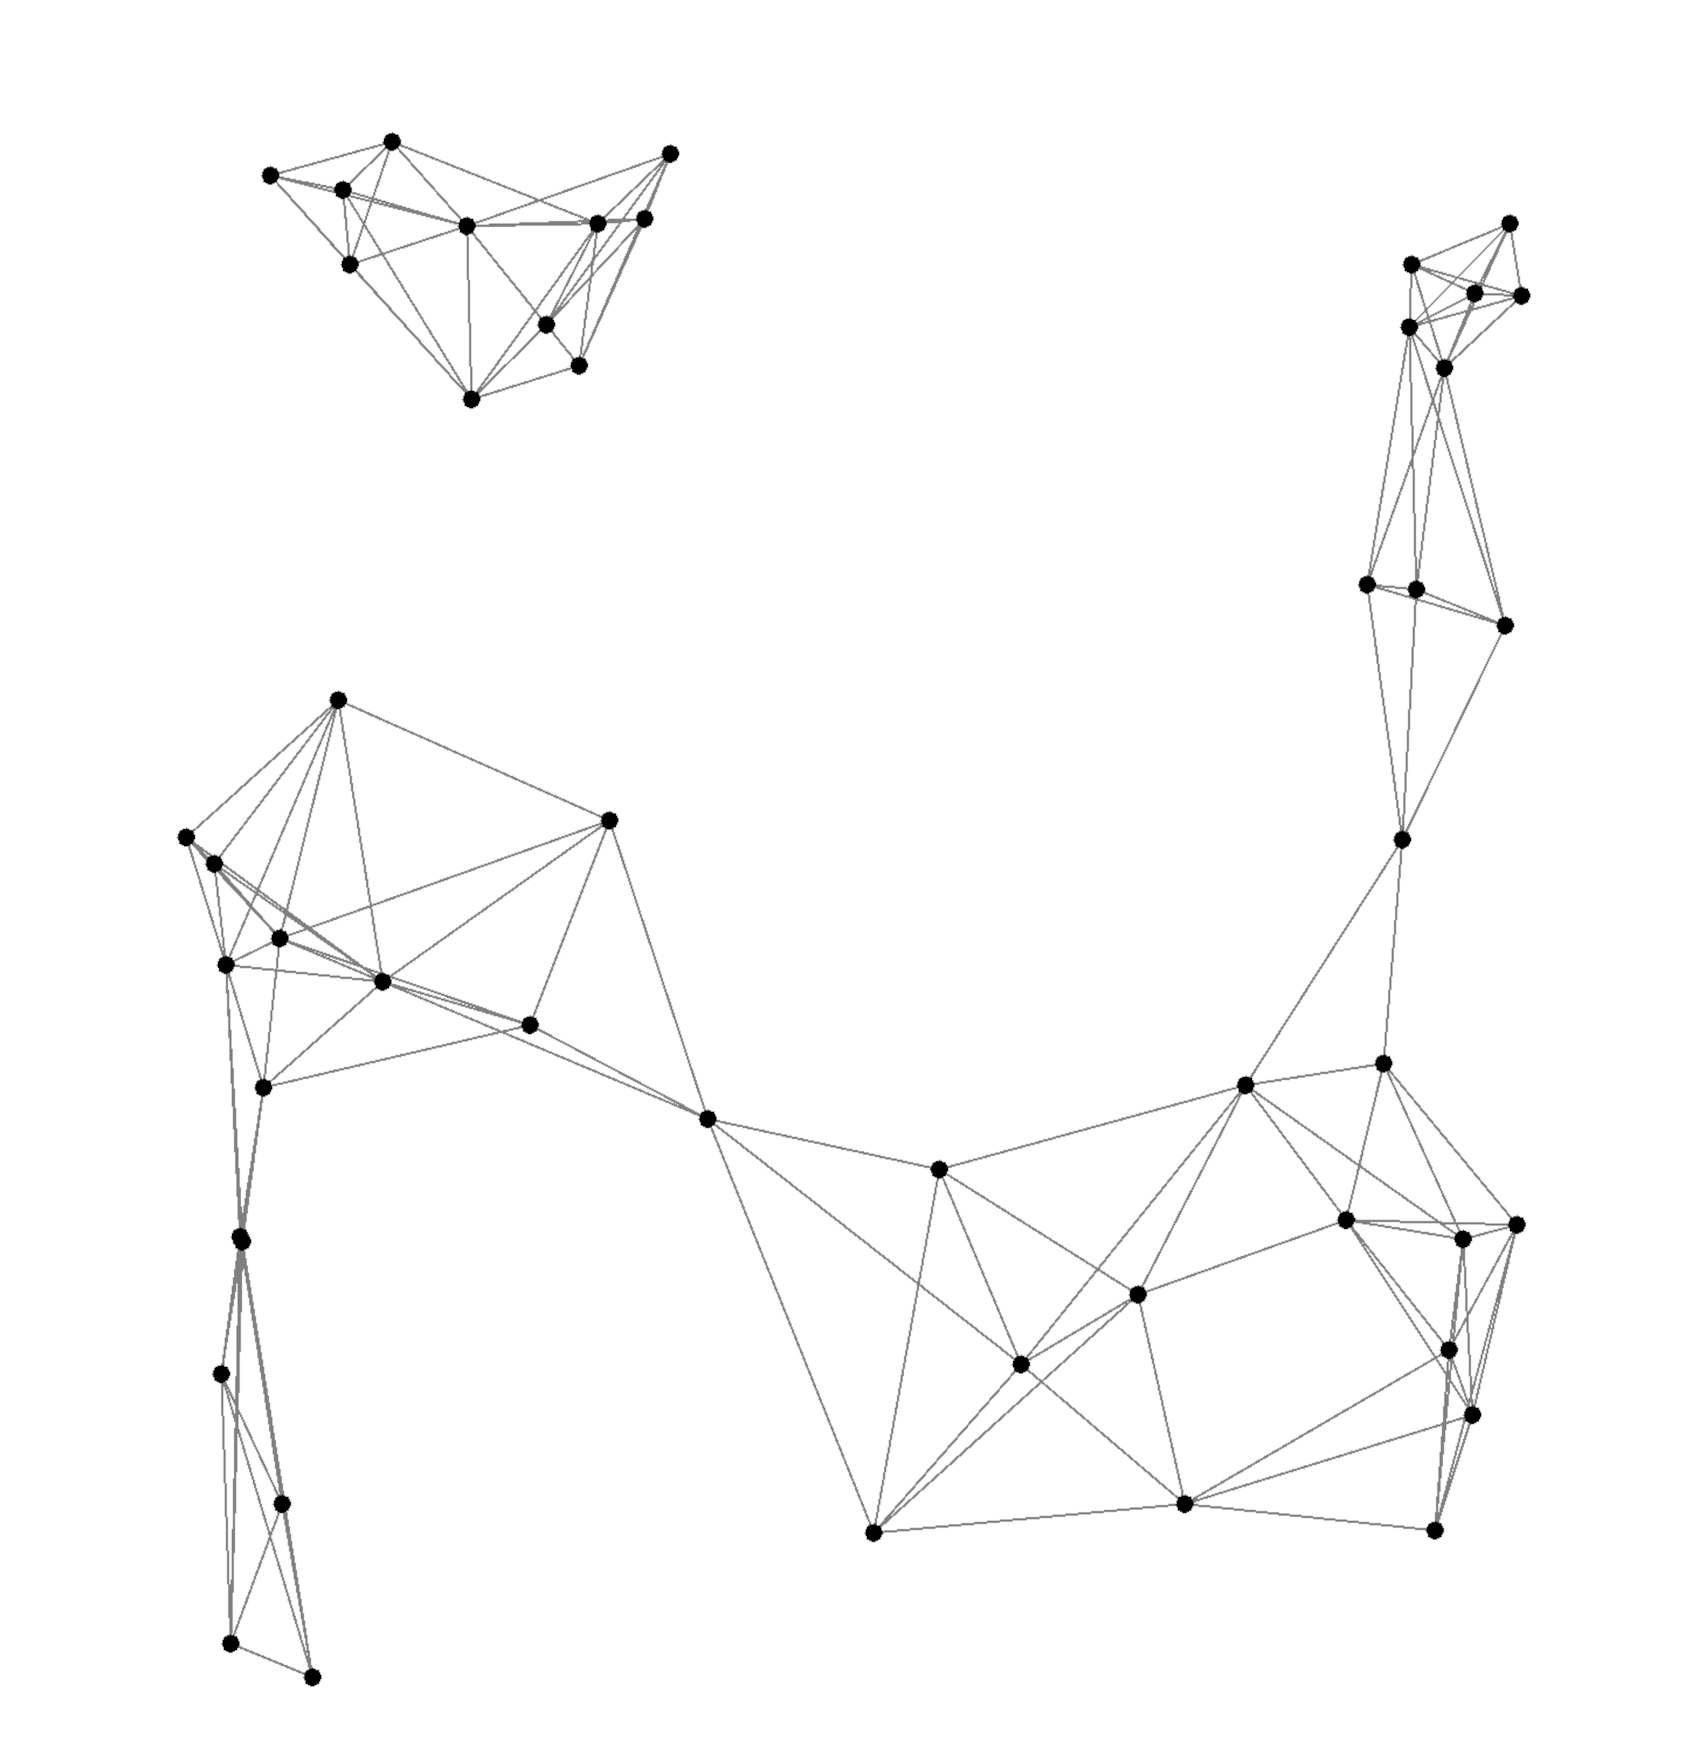
\includegraphics[width=\textwidth]{papers/coordination2023/imgs/4.png}}
        \caption{}
    \end{subfigure}
    \hfill
    \begin{subfigure}[b]{0.25\textwidth}
        \centering
        \fbox{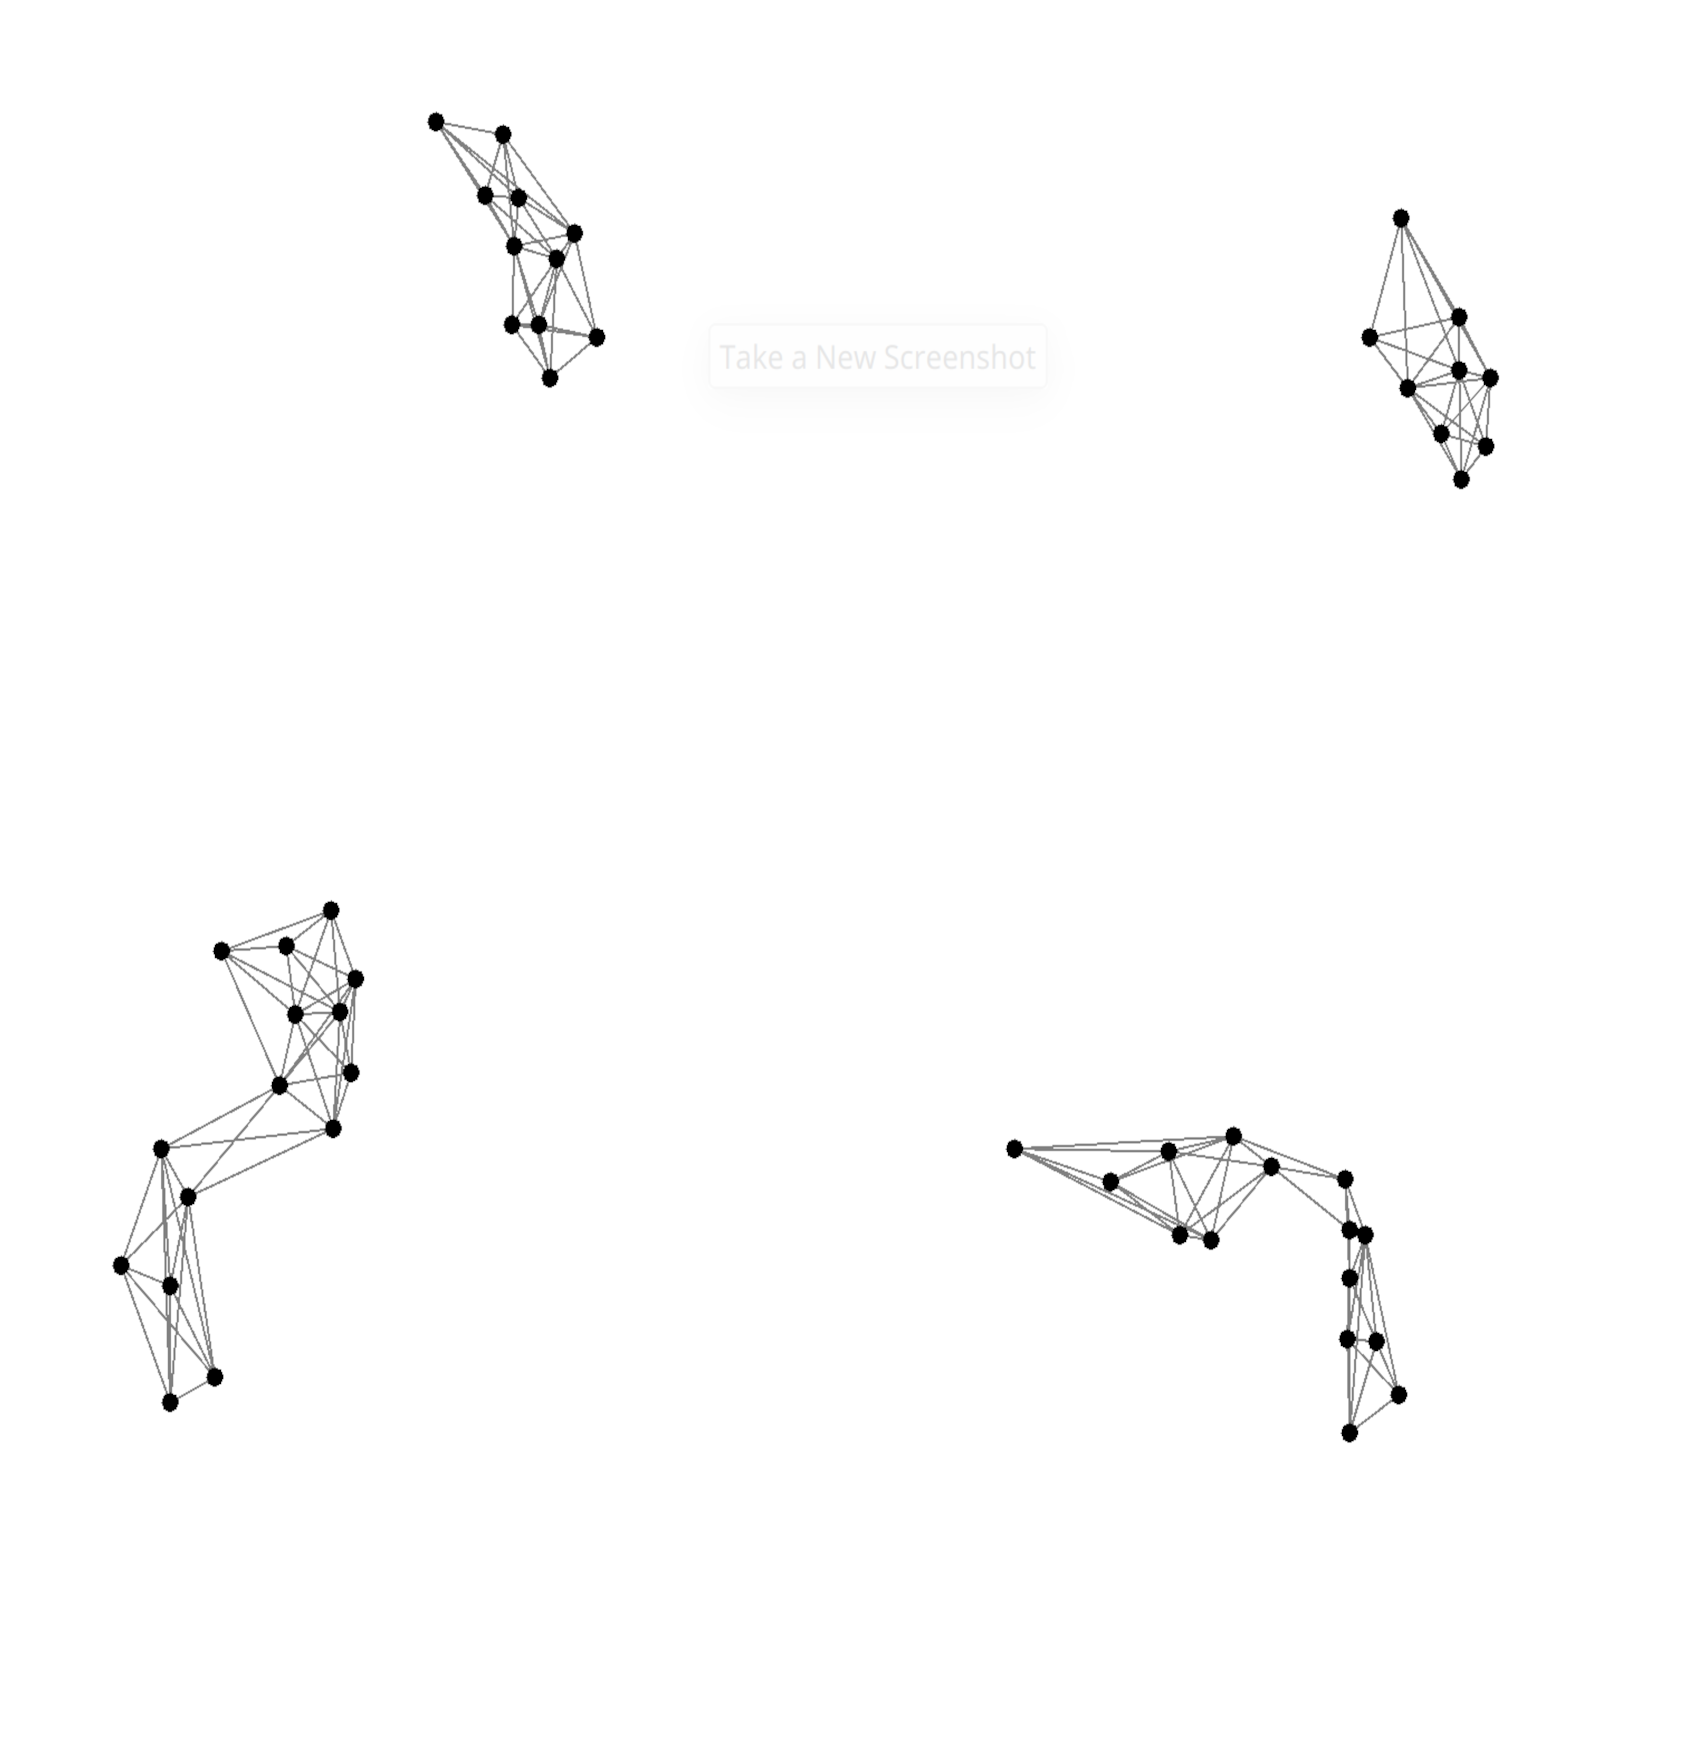
\includegraphics[width=\textwidth]{papers/coordination2023/imgs/7.png}}
        \caption{}
    \end{subfigure}
    \par
    \begin{subfigure}[b]{0.25\textwidth}
        \centering
        \fbox{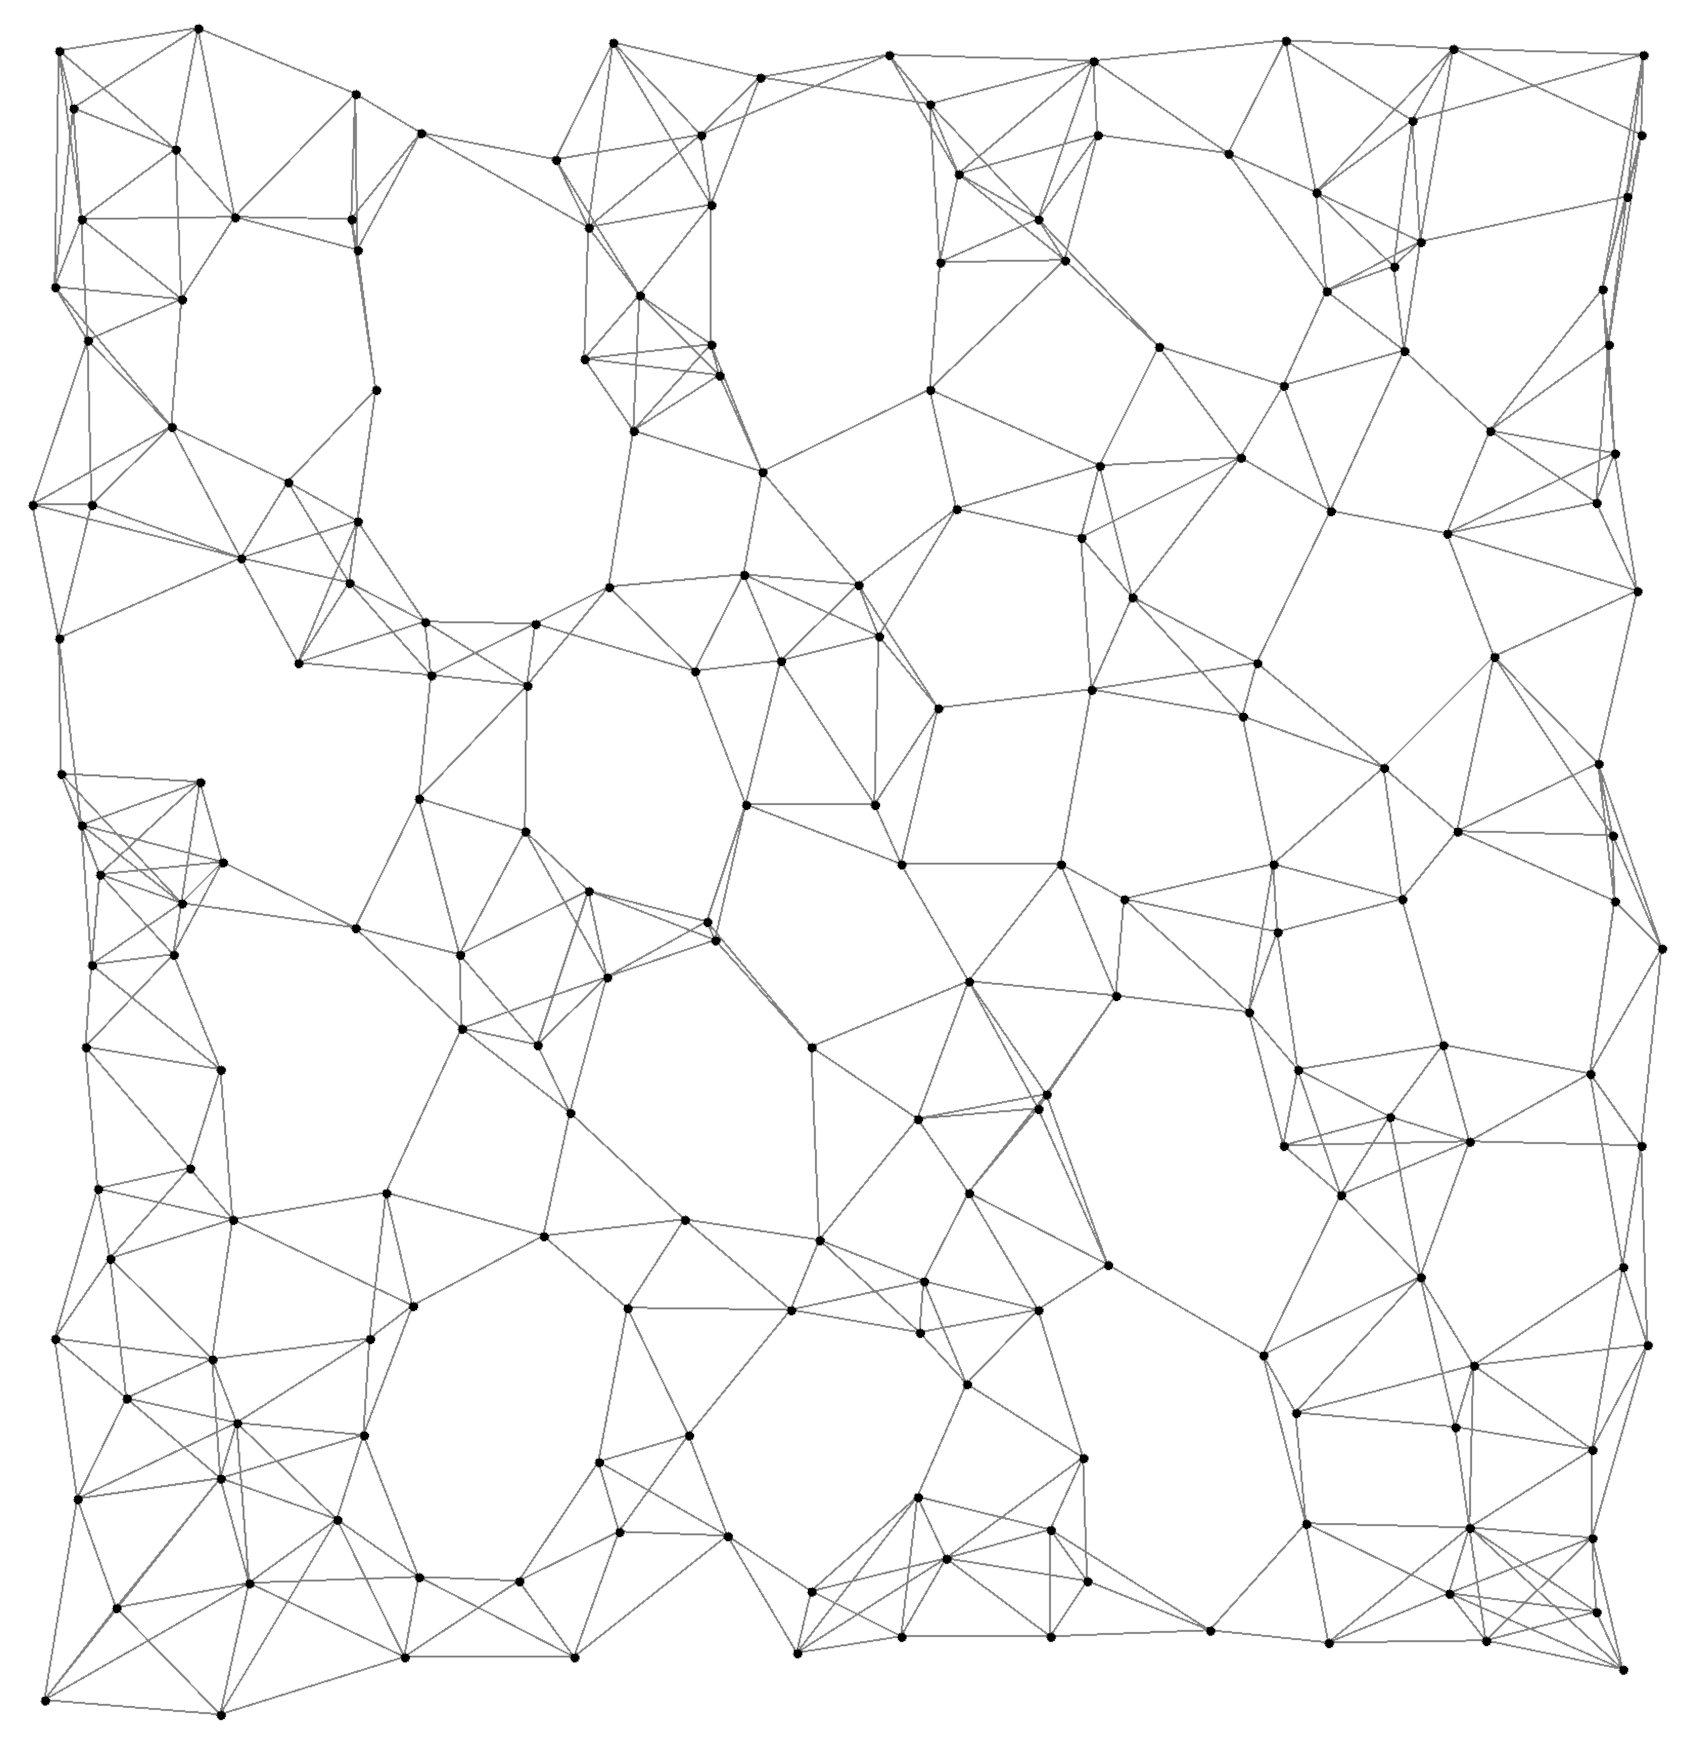
\includegraphics[width=\textwidth]{papers/coordination2023/imgs/1-large.png}}
        \caption{}
    \end{subfigure}
    \hfill
    \begin{subfigure}[b]{0.25\textwidth}
        \centering
        \fbox{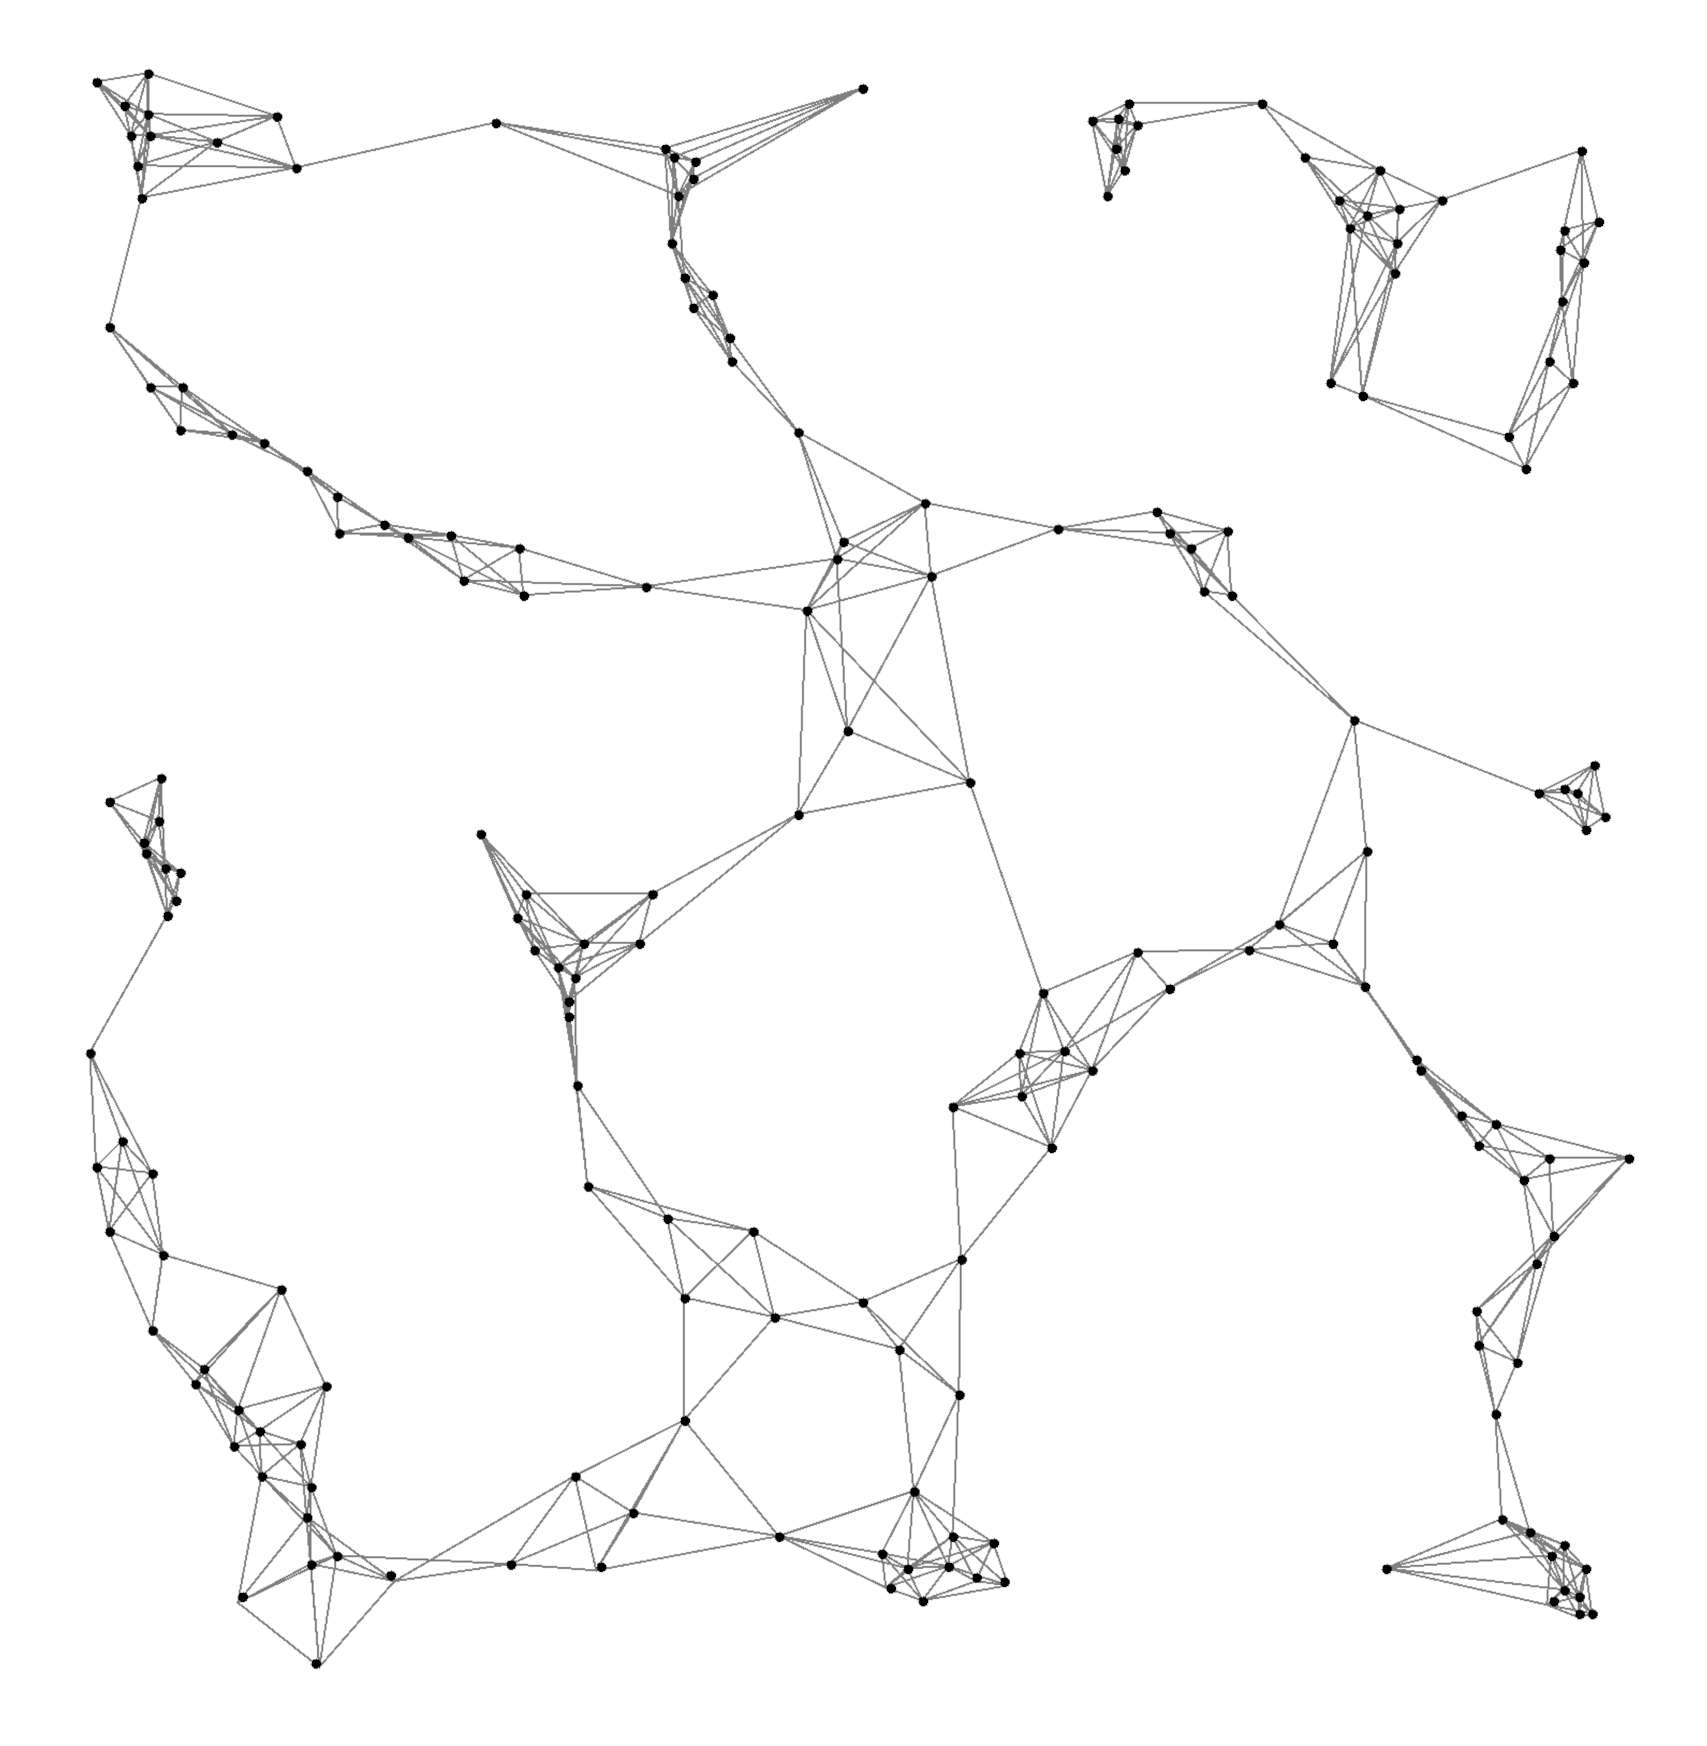
\includegraphics[width=\textwidth]{papers/coordination2023/imgs/3-large.png}}
        \caption{}
        \label{fig:sim2}
    \end{subfigure}
    \hfill
    \begin{subfigure}[b]{0.25\textwidth}
        \centering
        \fbox{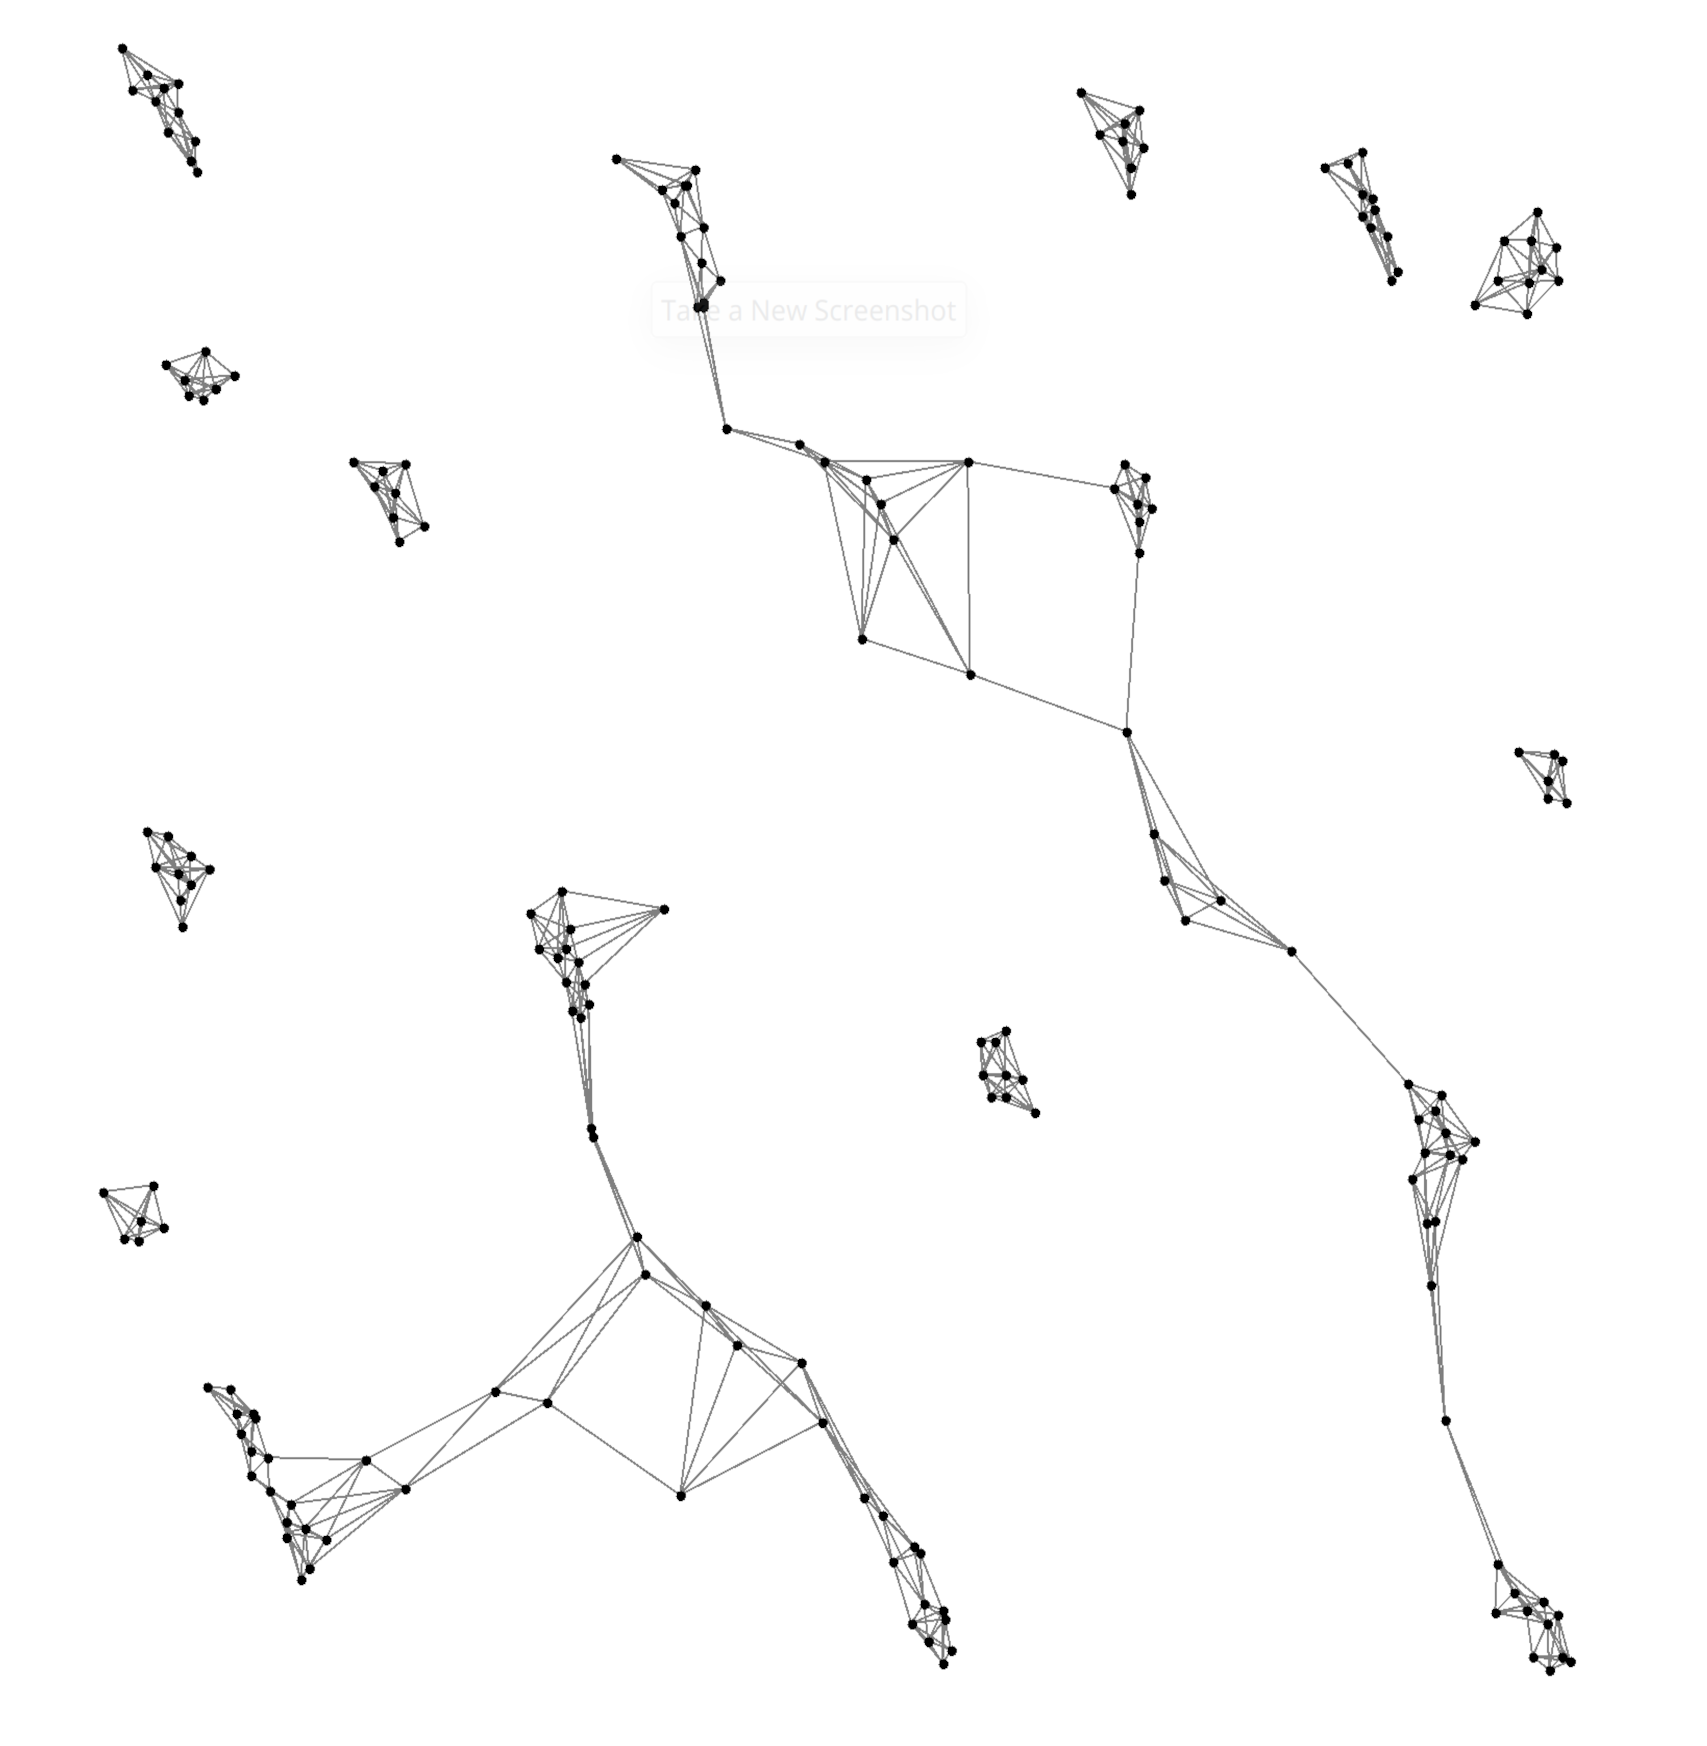
\includegraphics[width=\textwidth]{papers/coordination2023/imgs/4-large.png}}
        \caption{}
        \label{fig:sim3}
    \end{subfigure}
\caption[Snapshots of the learned policy in \scarlib{}]{Snapshots of the learned policy, the time flow is from left to right. 
In the first row, there are 50 agents, whereas in the second row, there are 200 agents.
In the last step of the simulation, the agents converged to a distance of approximately $\delta$.}
\label{fig:simulation-snapshots}
\end{figure*}

\begin{figure*}[h!]
    \centering
    \begin{subfigure}[b]{0.32\textwidth}
        \centering
        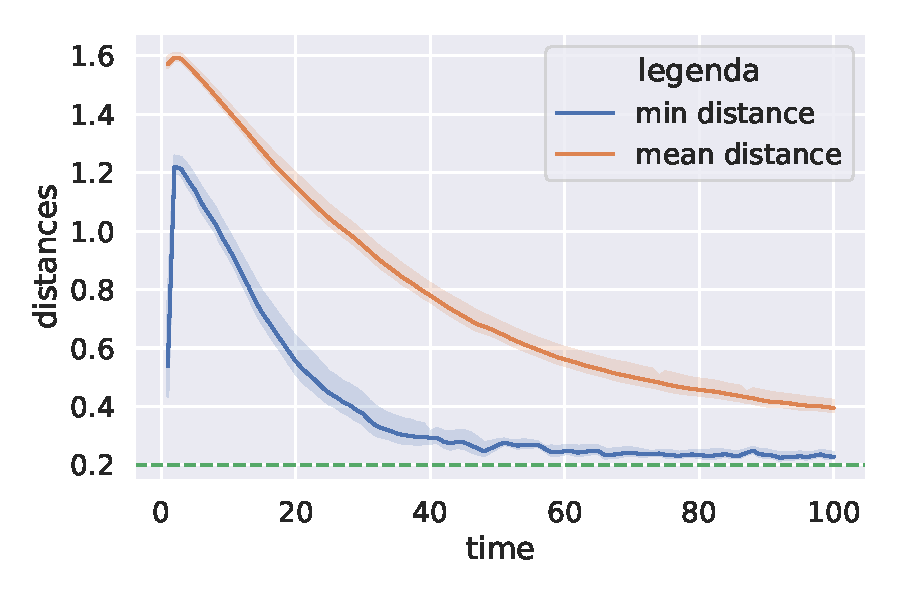
\includegraphics[width=\textwidth]{papers/coordination2023/imgs/data-50.pdf}
        \caption{50 agents}
    \end{subfigure}
    \hfill
    \begin{subfigure}[b]{0.32\textwidth}
        \centering
        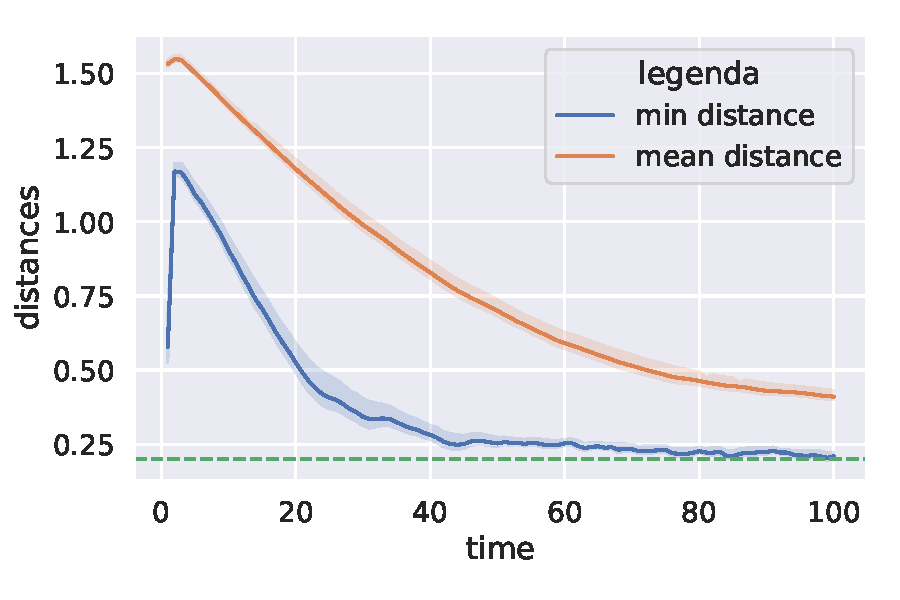
\includegraphics[width=\textwidth]{papers/coordination2023/imgs/data-100.pdf}
        \caption{100 agents}
    \end{subfigure}
    \hfill
    \begin{subfigure}[b]{0.32\textwidth}
        \centering
        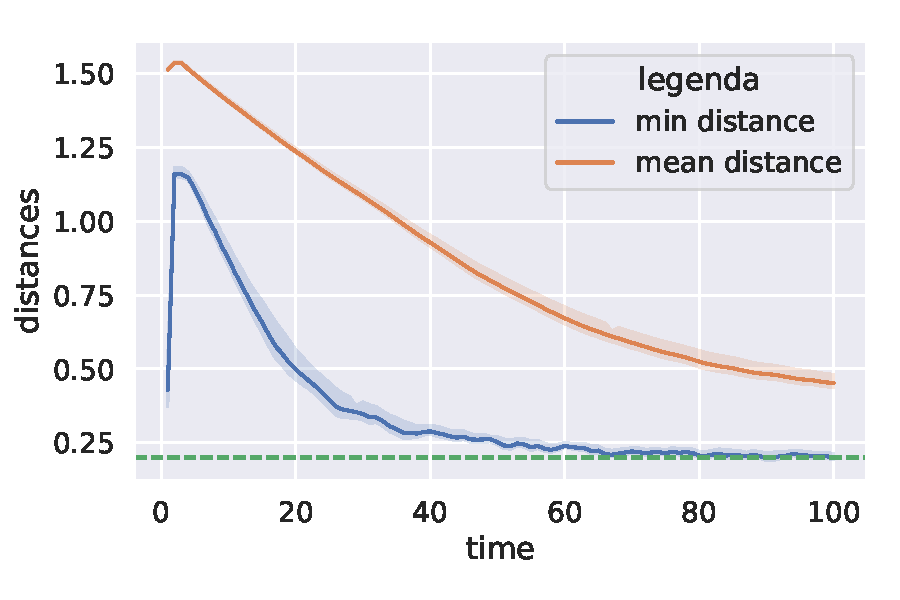
\includegraphics[width=\textwidth]{papers/coordination2023/imgs/data-200.pdf}
        \caption{200 agents}
    \end{subfigure}
\caption[The performance of the learned policy in \scarlib{}]{The performance of the learned policy. 
The y-axis represents the distance between the agents.
The x-axis represents the time.
The green line is equal to $\delta$.
In the charts, as the number of agents varies, the performance of the learned policy is similar.
Moreover, the minimum (blue line) distance between the agents is always greater than $\delta$.
The average distance (orange line) stays close to 2 * $\delta$ (after convergence).
}
\label{fig:test}
\end{figure*}
%\subsection*{Cleaning Robot}
%\paragraph{Description}
%This environment consists of N agents operating in a 2D world represented by a grid. 
% The world is discrete, and agents can move one step north, west, east, or south. 
% The world has a fixed size, so agents cannot move beyond the boundaries of the grid.
% The environment contains M dirty areas that need to be cleaned. 
%% The agents must learn to clean these areas efficiently and avoid unnecessarily 
 %cleaning areas that are already clean.
 %The agents will receive a reward for cleaning dirty areas and a penalty for cleaning clean areas.
 %More precisely, the reward function is:
%\begin{equation} % TODO: Update the reward function
%    r = \begin{cases}
%            +1 & \text{if the agent cleans a dirty area} \\
%            -1 & \text{if the agent cleans a clean area} \\
%            +100 & \text{if the room is clean} 
%    \end{cases}
%\end{equation}


%\paragraph{Results}
%Here you should show the result of the cleaning robot experiment
\section{Related work}\label{sec:related}
MARL has gained significant interest in the past decade, 
 leading to the development of several frameworks 
 for use in both research and industry communities. 
Here, we highlight current state-of-the-art solutions 
 for MARL problems and compare 
 them to the tools presented in this work.
\subsubsection{Many Agent simulators:}   
unlike supervised learning, 
 where a large dataset is required to improve neural network performance, 
 in RL, algorithms require a simulator to gain experience. 
One such comprehensive solution for MARL is PettingZoo~\cite{NEURIPS2021_7ed2d345}, 
 which provides both competitive and cooperative settings 
 for simulations with multiple agents. 
%
Another option for many-agent scenarios is NeuralMMO~\cite{https://doi.org/10.48550/arxiv.1903.00784}, 
 a GPU-optimized simulator for MMO-like games 
 that is designed to handle large-scale simulations of thousands of agents.
% 
Vectorized Multi-agent Simulator~\cite{bettini2022vmas} is another promising solution, 
 as it is optimized for collective tasks through GPU computation, 
 and it can be extended with additional environments.
%
While \scarlib is not directly linked to any simulator, 
 its main abstraction can be potentially linked 
 to both JVM-based simulators and gym-based Python environments. 
 Our choice of Alchemist was mainly due to its ability to express \ac{cmarl} settings easily, but potentially it can be used with any of the above-described solutions.
\subsubsection{Multi-Agent Deep RL libraries:}
since the importance of multi-agent settings several libraries have been developed in recent years. 
Ray~\cite{ray} is one of the most comprehensive frameworks, 
 originally designed for single-agent RL but 
 now integrated with basic concepts for MARL solutions thanks to MALib. 
It offers various MARL algorithms,
 supports different gym-like environments, 
 and is highly customizable through configuration files. 
%
PyMARL~\cite{samvelyan19smac} is one of the first solutions in Python for MARL, 
 though it is limited to specific algorithms (like VDN and QMIX), 
 and it is not generalizable. 
%
\scarlib{} is more similar to the first framework, 
 even though it is primarily designed for cooperative applications. 
%
However, since it was developed specifically for \ac{cmarl}, 
 it includes some abstractions and configurations that are not present in Ray, 
 such as the concept of a collective reward function and the configuration for CTDE. 
%
This reduces the time required to use \scarlib{} compared to Ray. 
 Additionally, \scarlib{} has a simple DSL that is easier to use than Ray's configuration system and is aided by the type system.

Finally, some innovative approaches aim to scale solutions to large populations of cooperative agents, such as mean-field RL. However, only a few implementations currently exist, and they are not considered to be general-purpose. \scarlib{}, on the other hand, offers a practical, simple implementation that can be leveraged in \ac{cmarl} settings.

Overall, \ac{cmarl} is a high-level framework that reduces the effort required for developers and practitioners to define and implement \ac{cmarl} problems when compared to current state-of-the-art solutions.

\subsubsection{Many-Agent Proof of Concept:}
the above RL library solutions are mainly created for multi-agent systems, 
 so they generally do not scale well with large populations of agents. 
 Novel approaches aim to scale the solution to potentially infinite populations of cooperative agents. 
In particular, mean-field RL~\cite{meanfield} is probably one of the 
 most interesting solutions in this context, 
 as it abstracts over the entire agent population 
 by considering only the average response of the neighbourhood. 
%
Currently, however, only a few implementations 
 exist~\footnote{\url{https://github.com/mlii/mfrl}} and they are not considered to be general-purpose. 
 \scarlib{} instead is practical and already provides a simple implementation that can be leveraged in \ac{cmarl} settings. 
\section{Conclusion and Future work}\label{conclusion}
In this paper, we presented \scarlib{}: 
 a collaborative many-agent deep reinforcement learning framework that integrates the functionalities of \scafi{} and Alchemist.
%
 The framework enables the definition of simulations of large-scale distributed scenarios 
 and the creation of complex scenarios with ease through its exposed DSL. 
% 
With \scarlib{}, developers can effectively and efficiently simulate and experiment with different reinforcement learning algorithms, 
 thereby providing a valuable tool for the advancement of coordination and multi-agent systems research.
Looking forward, \scarlib{} presents a promising solution 
 for expressing collaborative multi-agent reinforcement learning applications -- like hybrid aggregate computing solutions~\cite{Aguzzi2021,Aguzzi2022,Aguzzi2022-Roadmap,DBLP:conf/acsos/AguzziCV22}.
 However, further development and integration is necessary for it to be more easily adopted by non-expert users. 
 One area of improvement would be to integrate additional learning algorithms such as MAPPO~\cite{mappo} and mean field reinforcement learning~\cite{meanfield}, 
 as DQN is only a baseline approach.
%
Another aspect to be considered is the potential bottleneck that Alchemist may create during the learning phase since it is a JVM-based systems. 
%
To address this, we propose integrating a new environment, FLAME GPU~\cite{flame}, 
which has the ability to run entirely on GPU, 
thus providing faster learning and reducing the computational load. 
%
This integration would further enhance the capabilities of \scarlib{} and make it a more practical and efficient tool for \ac{cmarl} research.

%\subsubsection{Acknowledgements} Please place your acknowledgments at
%the end of the paper, preceded by an unnumbered run-in heading (i.e.
%3rd-level heading).


%
% ---- Bibliography ----
%
% BibTeX users should specify bibliography style 'splncs04'.
% References will then be sorted and formatted in the correct style.
%
\printbibliography